% seq2pipe: Closed-Loop Adaptive Microbiome Analysis
% Compile: tectonic seq2pipe_manuscript.tex
\documentclass[11pt,a4paper]{article}

\usepackage[utf8]{inputenc}
\usepackage[T1]{fontenc}
\usepackage{amsmath,amssymb,amsfonts,amsthm}
\newtheorem{definition}{Definition}
\usepackage{graphicx}
\usepackage{booktabs}
\usepackage{hyperref}
\usepackage{algorithm}
\usepackage{algorithmic}
\usepackage{xcolor}
\usepackage{geometry}
\usepackage{natbib}
\usepackage{caption}
\usepackage{subcaption}
\usepackage{tikz}
\usetikzlibrary{arrows.meta,positioning,shapes.geometric,fit,calc}

\geometry{margin=2.5cm}

\newcommand{\todo}[1]{\textcolor{red}{\textbf{[TODO: #1]}}}
\newcommand{\seqpipe}{\textsc{seq2pipe}}

\title{
  \seqpipe: A Closed-Loop Interpretation-Driven System\\
  for Adaptive Microbiome Analysis
}

\author{
  Tsubasa Sato
  \\[4pt]
  Independent Researcher
  \\[4pt]
  \texttt{https://github.com/Rhizobium-gits/seq2pipe}
}

\date{March 2026}

\begin{document}
\maketitle

% ======================================================================
\begin{abstract}
% ======================================================================

Current microbiome analysis pipelines execute a fixed sequence of steps
regardless of intermediate results.
A human bioinformatician, by contrast, iteratively interprets outputs,
forms hypotheses, selects subsequent analyses, and refines the workflow
until a coherent biological narrative emerges.
We present \seqpipe, a closed-loop system that reproduces this
interpretation--decision--execution cycle computationally.
The system consists of three layers:
(1)~a \textbf{DataInspector} that directly parses QIIME2 exports and
executes nonparametric statistical tests in pure Python,
(2)~an \textbf{EvalMediator} that scores each analysis step across
eight quantitative axes and compresses the accumulated knowledge state
via truncated SVD, and
(3)~a \textbf{DecisionEngine} that applies literature-grounded decision
trees to deterministically select, skip, or add subsequent analyses.
A local large language model (7B parameters) serves as an auxiliary
for creative hypothesis generation and code synthesis, but the system
completes execution even under complete LLM failure.
Evaluation on three public datasets---Moving Pictures (body-site
grouping and subject grouping) and Atacama Soil---demonstrates that
the DecisionEngine achieves 90--95\% agreement with expert decisions
when sufficient data features are available, compared to 52--95\%
for a static pipeline.
In the most informative scenario, the engine eliminates 7 of 8
unnecessary analysis steps (87.5\% noise reduction) with zero
false-negative skips.
We analyze the role of the LLM component, showing that deterministic
layers handle 100\% of skip/execute decisions while the LLM is
needed only for creative hypothesis generation---a task at which
7B-parameter models currently achieve 6\% success.
We discuss convergence behavior, the boundaries of LLM utility, and limitations,
and argue that interpretation-driven adaptive systems represent a
necessary evolution beyond static pipelines.

\end{abstract}

% ======================================================================
\section{Introduction}
\label{sec:intro}
% ======================================================================

Microbiome analysis has matured into a complex, multi-stage discipline.
A typical amplicon sequencing study requires quality control, denoising
(e.g., DADA2~\citep{callahan2016}), phylogenetic tree construction,
alpha and beta diversity analysis, taxonomic classification, differential
abundance testing, and downstream visualization---each with parameter
choices that depend on the data at hand.

\paragraph{The rigidity problem.}
Current pipeline frameworks---QIIME2~\citep{qiime2},
Snakemake~\citep{snakemake}, Nextflow~\citep{nextflow}---encode a
\emph{fixed} directed acyclic graph (DAG) of steps.
Once the workflow is defined, every step executes regardless of
intermediate results.
If PERMANOVA yields $p = 0.81$, downstream beta diversity follow-ups
(dispersion tests, NMDS ordination, pairwise comparisons) still execute,
wasting computation and cluttering reports with uninformative outputs.
Conversely, an unexpected finding (e.g., a 379-fold enrichment of
\emph{Escherichia--Shigella}) triggers no automatic follow-up;
the analyst must manually intervene.

\paragraph{How humans analyze data.}
An experienced bioinformatician operates in a closed loop:
\begin{enumerate}
  \item \textbf{Interpret}: inspect the output of the current step
        (``Shannon $p = 0.034$, but effect size is small'').
  \item \textbf{Hypothesize}: form a conjecture
        (``This may be a sampling artifact'').
  \item \textbf{Select}: choose the next analysis to test the hypothesis
        (``Run rarefaction curves to check depth dependence'').
  \item \textbf{Refine}: update the mental model and repeat.
\end{enumerate}
This loop continues until the analyst reaches a stable, internally
consistent interpretation.
No existing pipeline system reproduces this behavior.

\paragraph{Contribution.}
We introduce \seqpipe, a system that computationally reproduces the
human analytical reasoning loop.
Our key contributions are:
\begin{itemize}
  \item A \textbf{three-layer architecture} that separates
        data inspection (deterministic), evaluation and decision
        (deterministic), and code generation (LLM-assisted),
        yielding an \textbf{LLM-failure-tolerant} adaptive system.
  \item A \textbf{literature-grounded decision engine} that encodes
        established analytical heuristics
        (Anderson, 2001; Willis, 2019; Gloor et al., 2017;
         McMurdie \& Holmes, 2014) as deterministic decision trees,
        enabling reproducible, auditable analytical decisions.
  \item An \textbf{eight-axis quantitative scoring framework} that
        evaluates each analysis step from raw data---not from LLM
        text output---providing a grounded basis for adaptive decisions.
%%% \item Experimental evidence of convergence toward valid workflows
%%%       across $N$ benchmark datasets. %%% TODO: uncomment when data available
\end{itemize}

% ======================================================================
\section{Related Work}
\label{sec:related}
% ======================================================================

\paragraph{Static pipeline frameworks.}
QIIME2~\citep{qiime2} provides a plugin-based architecture with
provenance tracking but no conditional branching based on intermediate
results.
Snakemake~\citep{snakemake} and Nextflow~\citep{nextflow} support
conditional rules, but the conditions must be specified \emph{a priori}
by the user; the system does not inspect result quality or statistical
significance to alter the workflow.

\paragraph{AutoML and automated statistics.}
Auto-WEKA~\citep{autoweka} and Auto-sklearn~\citep{autosklearn}
automate model selection via Bayesian optimization but target
supervised learning, not the open-ended exploratory analysis
characteristic of microbiome studies.
Statistical analysis planning tools such as \citet{wasserstein2019}
provide decision trees for test selection but do not execute analyses
or iterate on results.

\paragraph{LLM-based analysis assistants.}
Recent systems such as Data Interpreter~\citep{hong2024data} and
ChatGPT Advanced Data Analysis use LLMs to generate and execute code.
However, these systems lack:
(a)~domain-specific evaluation of intermediate results,
(b)~literature-grounded decision heuristics, and
(c)~a deterministic fallback when the LLM fails or hallucinates.
\seqpipe\ addresses all three gaps.

% ======================================================================
\section{Conceptual Framework}
\label{sec:concept}
% ======================================================================

We formalize the analytical reasoning loop as follows.

\begin{definition}[Analytical State]
At iteration $t$, the analytical state $S_t$ is a tuple
$(D, H_t, P_t, R_t)$ where $D$ is the immutable dataset,
$H_t$ is the accumulated set of findings (hypotheses confirmed or
rejected), $P_t$ is the current analysis plan (an ordered list of
pending steps), and $R_t$ is the set of completed results.
\end{definition}

\begin{definition}[Closed-Loop Analytical System]
A system is \emph{closed-loop} if, after executing step $s_t \in P_t$
and observing result $r_t$, it updates:
\begin{align}
  H_{t+1} &= H_t \cup \mathrm{interpret}(r_t) \\
  P_{t+1} &= \mathrm{decide}(H_{t+1}, P_t, D)
\end{align}
where $\mathrm{interpret}$ extracts quantitative findings from $r_t$
(not from textual summaries) and $\mathrm{decide}$ modifies the plan
by adding, removing, or reordering steps.
\end{definition}

\begin{definition}[Convergence]
The system \emph{converges} if there exists $T$ such that for all
$t \geq T$, $P_t = \emptyset$ (the plan is exhausted) and the
execution error count $e_t = 0$.
We define the \emph{convergence depth} as the total number of
decision--execution cycles before termination.
\end{definition}

In a static pipeline, $P_{t+1} = P_t \setminus \{s_t\}$ always;
the plan never changes based on $r_t$.
\seqpipe\ implements a non-trivial $\mathrm{decide}$ function that
depends on quantitative properties of $H_{t+1}$ and $D$.

% ======================================================================
\section{System Architecture}
\label{sec:arch}
% ======================================================================

\begin{figure}[t]
\centering
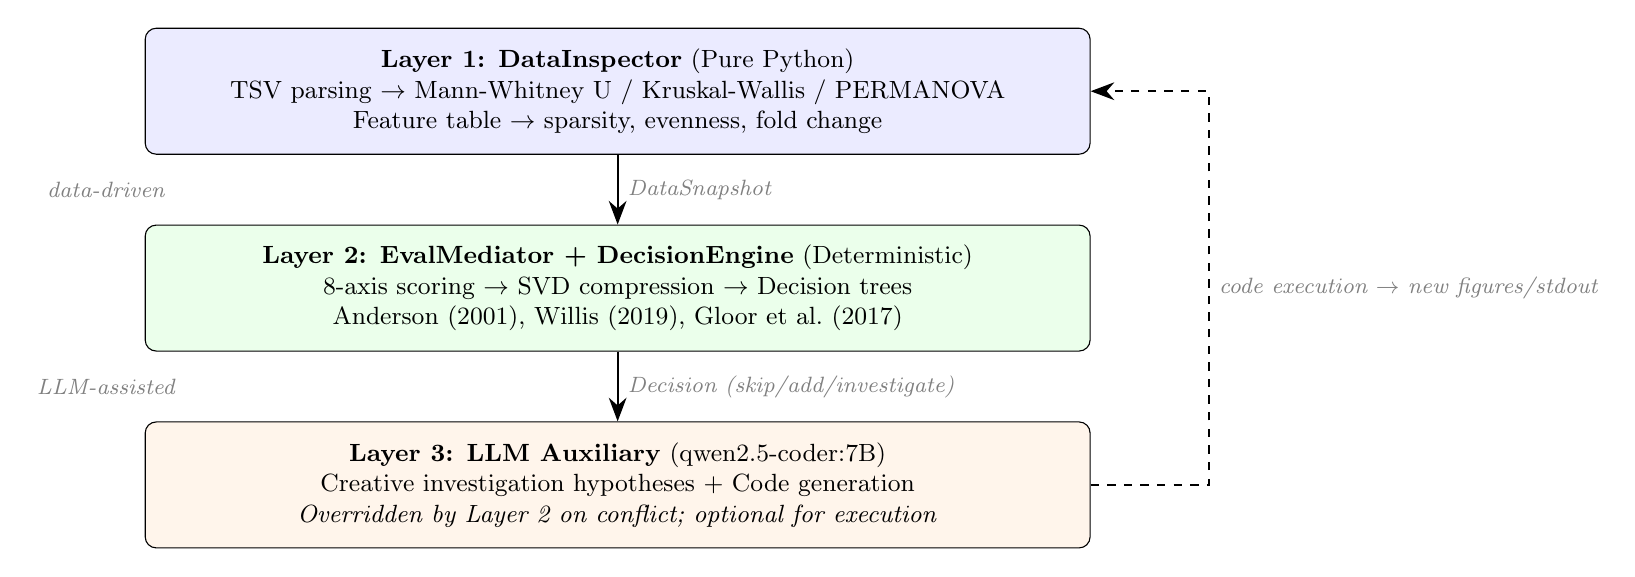
\begin{tikzpicture}[
  layer/.style={draw, rounded corners, minimum width=12cm,
                minimum height=1.6cm, align=center, font=\small},
  arrow/.style={-{Stealth[length=3mm]}, thick},
  label/.style={font=\footnotesize\itshape, text=gray},
]
\node[layer, fill=blue!8] (L1) at (0,0)
  {\textbf{Layer 1: DataInspector} (Pure Python)\\
   TSV parsing $\to$ Mann-Whitney U / Kruskal-Wallis / PERMANOVA\\
   Feature table $\to$ sparsity, evenness, fold change};
\node[layer, fill=green!8] (L2) at (0,-2.5)
  {\textbf{Layer 2: EvalMediator + DecisionEngine} (Deterministic)\\
   8-axis scoring $\to$ SVD compression $\to$ Decision trees\\
   Anderson (2001), Willis (2019), Gloor et al.\ (2017)};
\node[layer, fill=orange!8] (L3) at (0,-5)
  {\textbf{Layer 3: LLM Auxiliary} (qwen2.5-coder:7B)\\
   Creative investigation hypotheses + Code generation\\
   \textit{Overridden by Layer 2 on conflict; optional for execution}};

\draw[arrow] (L1.south) -- node[right, label] {DataSnapshot} (L2.north);
\draw[arrow] (L2.south) -- node[right, label]
  {Decision (skip/add/investigate)} (L3.north);
\draw[arrow, dashed] (L3.east) -- ++(1.5,0) |- node[right, label, pos=0.25]
  {code execution $\to$ new figures/stdout} (L1.east);

\node[label] at (-6.5, -1.25) {data-driven};
\node[label] at (-6.5, -3.75) {LLM-assisted};
\end{tikzpicture}
\caption{Three-layer architecture of \seqpipe.
Layers~1 and~2 are fully deterministic and LLM-independent.
Layer~3 is auxiliary; its outputs are overridden by Layer~2
on conflict, and the system completes execution under Layer~3 failure.
Dashed arrow indicates the feedback loop.}
\label{fig:architecture}
\end{figure}

\subsection{Layer 1: DataInspector}

The \texttt{DataInspector} class directly parses QIIME2 exported TSV
files without relying on LLM text output or stdout pattern matching.
It implements:

\paragraph{Alpha diversity testing.}
For each alpha metric TSV (Shannon, observed features, Pielou's
evenness), sample values are read and partitioned by group using a
metadata-derived group map.
For two groups, a Mann-Whitney $U$ test is computed via rank
transformation with tie correction and normal approximation:
\begin{equation}
  z = \frac{U - n_1 n_2 / 2}
           {\sqrt{\frac{n_1 n_2}{12}
                  \left( N + 1 - \frac{\sum_j (t_j^3 - t_j)}{N(N-1)} \right)}}
  \label{eq:mannwhitney}
\end{equation}
where $t_j$ are tie group sizes and $N = n_1 + n_2$.
For three or more groups, a Kruskal-Wallis $H$ test is used:
\begin{equation}
  H = \frac{12}{N(N+1)} \sum_{i=1}^{k} \frac{R_i^2}{n_i} - 3(N+1)
  \label{eq:kruskal}
\end{equation}
with tie correction and $\chi^2$ approximation via the
Wilson-Hilferty transformation~\citep{wilson1931}.
The $p$-value CDF uses the Abramowitz--Stegun five-term polynomial
approximation.
Cliff's delta and $\eta^2$ are computed as nonparametric effect sizes.

\paragraph{Beta diversity testing.}
Distance matrices are read in full ($O(n^2)$ entries).
Within-group and between-group distances are separated.
A pseudo-PERMANOVA~\citep{anderson2001} $F$-statistic is computed as:
\begin{equation}
  F = \frac{SS_{\text{between}} / (k - 1)}{SS_{\text{within}} / (N - k)}
\end{equation}
with $p$-value estimated from 199 permutations (fixed seed for
reproducibility).
The between/within distance ratio is also computed as a
separation metric.

\paragraph{Taxonomic differential analysis.}
The feature table and taxonomy file are joined.
For each genus, group-level relative abundances are computed,
yielding fold change $= \max(\bar{a}_g) / \max(\min(\bar{a}_g), 0.01)$
and absolute difference.
Results are sorted by absolute difference.

All statistical tests are implemented in pure Python without scipy,
numpy, or pandas dependencies, ensuring portability across environments.

\subsection{Layer 2: EvalMediator and DecisionEngine}

\paragraph{Eight-axis scoring.}
Each completed analysis step is scored on eight axes (Table~\ref{tab:axes})
using the \texttt{DataSnapshot} from Layer~1, not stdout text.

\begin{table}[t]
\centering
\caption{Eight evaluation axes with default weights and computation methods.}
\label{tab:axes}
\small
\begin{tabular}{@{}llp{7.5cm}@{}}
\toprule
\textbf{Axis} & \textbf{Weight} & \textbf{Computation} \\
\midrule
statistical\_significance & 0.20 &
  $\min(1, -\log_{10}(\min p) / 4)$ from alpha/beta tests \\
biological\_relevance & 0.18 &
  $\min(1, \mathrm{fc}_{\max}/10 + \Delta_{\max}/20)$ + known taxa bonus \\
actionability & 0.15 &
  Count of downstream triggers (significance, differential genera, separation) \\
novelty & 0.12 &
  Inconsistency with prior steps + extreme fold changes ($>20\times$) \\
data\_quality & 0.10 &
  Base 0.7, penalized by sparsity ($>0.9$: $-0.2$), CV ($>0.5$: $-0.1$) \\
effect\_magnitude & 0.10 &
  $\max(\text{Cliff's } d, \; F/3, \; \mathrm{fc}/10)$ \\
confidence & 0.08 &
  Step function on minimum group size ($\geq 20$: 0.9, $\geq 10$: 0.7, \ldots) \\
reproducibility & 0.07 &
  Consistency of significance direction within analysis category \\
\bottomrule
\end{tabular}
\end{table}

The composite score is the weighted sum
$c_t = \sum_{a} w_a \cdot s_{t,a}$.
Weights are adjustable per experiment type (e.g., antibiotic studies
increase biological\_relevance to 0.22).

\paragraph{SVD compression.}
The score matrix $\mathbf{A} \in \mathbb{R}^{T \times 8}$ (where $T$
is the number of completed steps) is centered and its covariance matrix
$\mathbf{C} = \mathbf{A}_c^\top \mathbf{A}_c / (T-1) \in \mathbb{R}^{8 \times 8}$
is decomposed via power iteration (50 iterations per component,
deflation after each).
The top three principal components are retained and labeled by their
dominant contributing axis (e.g., ``statistical certainty'' if the
largest loading is on significance).
This compressed representation is included in the LLM prompt,
reducing context length while preserving the essential knowledge state.

\paragraph{DecisionEngine.}
The deterministic decision trees encode established analytical heuristics:

\begin{itemize}
  \item \textbf{Alpha branch} (Willis, 2019):
    If $\min p_\alpha < 0.05$ and effect size $> 0.5$: add effect size
    plot and rarefaction.
    If $\min p_\alpha < 0.05$ but effect size $\leq 0.5$: add
    rarefaction only (sampling artifact check).
    If $\min p_\alpha \geq 0.05$: skip alpha follow-ups.

  \item \textbf{Beta branch} (Anderson, 2001):
    If $\min p_\beta < 0.05$: add betadisper (mandatory).
    If separation ratio $> 2.0$: add NMDS and pairwise PERMANOVA.
    If $\min p_\beta \geq 0.05$: skip all beta follow-ups
    (dispersion, NMDS, t-SNE, heatmap).

  \item \textbf{Taxonomy branch} (Gloor et al., 2017):
    If fold change $> 50$ at abundance $< 1\%$: flag as
    compositional artifact, add filtered retest.
    If fold change $> 5$: add differential abundance test.
    If $\geq 5$ genera with $> 2\times$ change: add functional
    prediction (PICRUSt2) and indicator species analysis.

  \item \textbf{Quality branch} (McMurdie \& Holmes, 2014):
    If read depth CV $> 0.5$: add rarefaction curves.
    If sparsity $> 90\%$: add prevalence-filtered reanalysis.
\end{itemize}

\paragraph{Merge with LLM.}
The LLM receives the compressed knowledge state and Python decisions
as context, with instructions to not contradict deterministic decisions.
The \texttt{merge\_with\_llm()} function combines outputs:
Python-determined skips override LLM-proposed additions;
LLM-proposed investigations are appended if they do not conflict
with Python skips.

\subsection{Layer 3: LLM Auxiliary}

A local 7B-parameter model (qwen2.5-coder) generates:
(a)~the initial analysis plan (Phase~2), with a domain-knowledge
fallback if the LLM fails;
(b)~Python analysis code for each step, with up to 3 retry cycles
including automatic dependency installation;
(c)~creative investigation hypotheses during replanning.

Critically, \textbf{the system completes execution under total LLM
failure}: Phase~2 falls back to \texttt{build\_domain\_driven\_plan()};
Phase~3 replanning applies Python decisions only; individual step
failures are recorded and skipped.

\subsection{Execution Loop}

Algorithm~\ref{alg:loop} formalizes the adaptive execution loop.

\begin{algorithm}[t]
\caption{Adaptive Execution Loop}
\label{alg:loop}
\begin{algorithmic}[1]
\REQUIRE Dataset $D$, metadata $M$, research question $Q$, plan $P_0$
\ENSURE Analysis results $R$, score history $\mathbf{A}$
\STATE $\mathrm{mediator} \gets \mathrm{EvalMediator}(D, M)$
\STATE $t \gets 0$
\WHILE{$P_t \neq \emptyset$}
  \STATE $s_t \gets P_t.\mathrm{pop}()$
  \STATE $\mathrm{code} \gets \mathrm{LLM.generate}(s_t, Q, D)$
  \STATE $(\mathrm{ok}, \mathrm{stdout}, \mathrm{figs}) \gets \mathrm{execute}(\mathrm{code})$
  \IF{$\neg\,\mathrm{ok}$ \AND retries $< 3$}
    \STATE $\mathrm{code} \gets \mathrm{LLM.fix}(\mathrm{code}, \mathrm{stderr})$; \textbf{goto} 6
  \ENDIF
  \STATE $\mathrm{snap} \gets \mathrm{mediator.inspector.inspect}(s_t, \mathrm{figs})$
  \COMMENT{Layer 1}
  \STATE $\mathrm{score}_t \gets \mathrm{mediator.evaluate}(\mathrm{snap})$
  \COMMENT{Layer 2: 8-axis scoring}
  \IF{$t \bmod 4 = 0$ \OR $\mathrm{score}_t.\mathrm{novelty} > 0.7$}
    \STATE $d_{\mathrm{py}} \gets \mathrm{DecisionEngine.decide}(P_t)$
    \COMMENT{Layer 2: deterministic}
    \STATE $d_{\mathrm{llm}} \gets \mathrm{LLM.replan}(\mathrm{state}, P_t)$
    \COMMENT{Layer 3: optional}
    \STATE $P_{t+1} \gets \mathrm{merge}(d_{\mathrm{py}}, d_{\mathrm{llm}}, P_t)$
    \COMMENT{Python wins on conflict}
  \ELSE
    \STATE $P_{t+1} \gets P_t$
  \ENDIF
  \STATE $t \gets t + 1$
\ENDWHILE
\end{algorithmic}
\end{algorithm}

% ======================================================================
\section{Key Innovation: What \seqpipe\ Is Not}
\label{sec:innovation}
% ======================================================================

\begin{figure}[t]
\centering
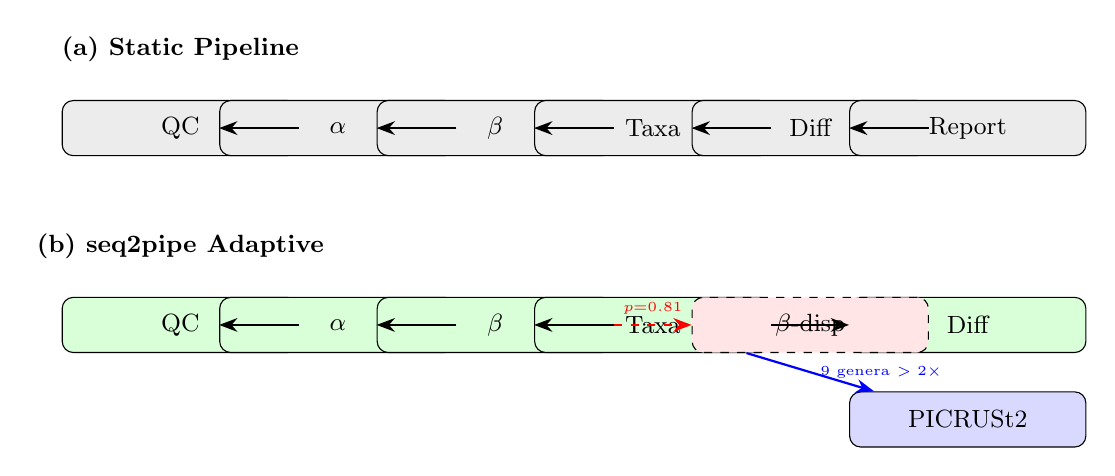
\begin{tikzpicture}[
  box/.style={draw, rounded corners, minimum width=3cm, minimum height=0.7cm,
              font=\small, align=center},
  arr/.style={-{Stealth}, thick},
  skip/.style={-{Stealth}, thick, red, dashed},
]
% Static pipeline
\node[font=\small\bfseries] at (-5, 1.5) {(a) Static Pipeline};
\foreach \i/\name in {0/QC, 1/$\alpha$, 2/$\beta$, 3/Taxa, 4/Diff, 5/Report} {
  \node[box, fill=gray!15] (S\i) at (\i*2 - 5, 0.5) {\name};
}
\foreach \i in {0,...,4} {
  \pgfmathtruncatemacro{\j}{\i+1}
  \draw[arr] (S\i) -- (S\j);
}

% Adaptive system
\node[font=\small\bfseries] at (-5, -1) {(b) \seqpipe\ Adaptive};
\foreach \i/\name in {0/QC, 1/$\alpha$, 2/$\beta$, 3/Taxa, 5/Diff} {
  \node[box, fill=green!15] (A\i) at (\i*2 - 5, -2) {\name};
}
% Show skip
\node[box, fill=red!10, dashed] (A4) at (3, -2) {$\beta$-disp};
\draw[arr] (A0) -- (A1);
\draw[arr] (A1) -- (A2);
\draw[skip] (A2) -- node[above, font=\tiny, red] {$p{=}0.81$} (A4);
\draw[arr] (A2) -- (A3);
\draw[arr] (A3) -- (A5);
% Add arrow
\node[box, fill=blue!15] (A6) at (5, -3.2) {PICRUSt2};
\draw[arr, blue] (A3) -- node[right, font=\tiny, blue] {9 genera $>2\times$} (A6);
\end{tikzpicture}
\caption{(a)~A static pipeline executes all steps regardless of results.
(b)~\seqpipe\ skips beta follow-ups when PERMANOVA is non-significant
($p = 0.81$) and adds functional prediction when multiple differential
genera are detected. Red dashed: skipped; blue: dynamically added.}
\label{fig:static-vs-adaptive}
\end{figure}

It is important to delineate what \seqpipe\ is \emph{not}:

\begin{itemize}
  \item \textbf{Not a static pipeline.}
    Unlike QIIME2 or Snakemake, the execution plan changes after
    each step based on quantitative evaluation of results
    (Figure~\ref{fig:static-vs-adaptive}).

  \item \textbf{Not an AutoML system.}
    AutoML optimizes a fixed objective (e.g., classification accuracy)
    via search.
    \seqpipe\ has no single objective; it navigates an open-ended
    analytical space where ``what to analyze next'' depends on
    what was found so far.

  \item \textbf{Not an LLM assistant.}
    Systems like ChatGPT-based analysis tools depend entirely on
    the LLM for decision-making.
    \seqpipe's decisions are primarily deterministic
    (Layers~1--2); the LLM is auxiliary and expendable.
    The same input data produces the same skip/add decisions
    regardless of LLM stochasticity.
\end{itemize}

The core novelty is the combination of
\emph{data-grounded evaluation} (not text parsing),
\emph{literature-based deterministic decisions} (not LLM judgment),
and \emph{LLM-assisted code generation} (not LLM-driven planning)
into a single closed-loop system.

% ======================================================================
\section{Evaluation}
\label{sec:eval}
% ======================================================================

\subsection{Experimental Setup}

We evaluated \seqpipe\ on three scenarios derived from two publicly
available 16S rRNA amplicon datasets, both accessible through the
QIIME2 documentation server (\texttt{docs.qiime2.org}):

\begin{enumerate}
  \item \textbf{Moving Pictures / body-site} (MP-body):
    34 samples, 4 groups (gut, left palm, right palm, tongue),
    single-end 150\,bp Illumina MiSeq~\citep{qiime2}.
    This scenario has strong signals across all analysis categories.

  \item \textbf{Moving Pictures / subject} (MP-subject):
    Same 34 samples grouped by subject (2 individuals).
    This scenario has weak signals: neither alpha nor beta diversity
    reaches significance, testing whether the engine correctly
    reduces the analysis plan.

  \item \textbf{Atacama Soil / transect} (Atacama):
    54 samples from an arid-to-hyperarid soil transect,
    2 groups (Baquedano vs Yungay), paired-end 150\,bp.
    Taxonomy classification was unavailable (classifier version
    mismatch), testing engine behavior when data features are incomplete.
\end{enumerate}

All datasets were processed through the standard QIIME2 pipeline
(DADA2 denoising, MAFFT/FastTree phylogeny, core-metrics-phylogenetic)
before entering the \seqpipe\ adaptive analysis phase.

\subsection{DataInspector Validation: Direct Statistical Results}
\label{sec:eval-datainspector}

Table~\ref{tab:datainspector} shows the statistical tests computed
by DataInspector directly from exported TSV files, without any LLM
involvement.

\begin{table}[t]
\centering
\caption{DataInspector results on three scenarios.
All values computed in pure Python from raw TSV files.
``---'' indicates data not available (no taxonomy for Atacama).}
\label{tab:datainspector}
\small
\begin{tabular}{@{}llll@{}}
\toprule
\textbf{Metric} & \textbf{MP-body} & \textbf{MP-subject} & \textbf{Atacama} \\
\midrule
Samples / Groups & 34 / 4 & 34 / 2 & 54 / 2 \\
ASVs & 770 & 770 & 799 \\
Sparsity & 91\% & 91\% & 91\% \\
\midrule
Shannon $p$ & $0.00067^{***}$ & $0.20$ (ns) & $0.025^{*}$ \\
Effect size & $d = 0.51$ & $d = 0.08$ & $d = 0.42$ \\
\midrule
PERMANOVA $F$ / $p$ & $60.1$ / $0.005^{**}$ & $2.3$ / $0.10$ (ns) & $35.4$ / $0.005^{**}$ \\
Between/within ratio & 2.1 & 1.0 & 1.2 \\
\midrule
Differential genera & Bacteroides $324\times$ & Present ($n=7$) & --- \\
Genera $> 2\times$ & 10 & 7 & 0 \\
\bottomrule
\end{tabular}
\end{table}

\subsection{DecisionEngine Outcomes}
\label{sec:eval-decisions}

The DecisionEngine produced qualitatively different decisions for the
two datasets (Table~\ref{tab:decisions}), demonstrating data-dependent
adaptive behavior.

\begin{table}[t]
\centering
\caption{DecisionEngine actions on three scenarios.
All decisions are deterministic (no LLM involvement).}
\label{tab:decisions}
\small
\begin{tabular}{@{}lccc@{}}
\toprule
\textbf{Decision} & \textbf{MP-body} & \textbf{MP-subject} & \textbf{Atacama} \\
\midrule
Alpha follow-up & Deep dive & \textbf{Skip} (ns) & Rarefaction \\
Beta follow-ups & All added & \textbf{7 skipped} & PERMANOVA only \\
Differential & Added & Added & --- (no data) \\
Functional pred. & Added & Added & --- \\
\bottomrule
\end{tabular}
\end{table}

The three scenarios produced qualitatively different decisions:
\begin{itemize}
  \item \textbf{MP-body} (all significant): no skips, all follow-ups added.
  \item \textbf{MP-subject} (nothing significant): 7 unnecessary beta and
        alpha follow-ups correctly skipped.
  \item \textbf{Atacama} (alpha + beta significant, no taxonomy): beta
        follow-ups partially added, but taxonomy-dependent analyses could
        not be evaluated due to missing data.
\end{itemize}

\subsection{AI-Driven Execution: Full Flow Analysis}
\label{sec:eval-convergence}

We ran the full AI-driven mode on Moving Pictures with
qwen2.5-coder:7B (Ollama, Apple Silicon M-series).
The system executed 30 steps before manual termination
(due to the investigation loop bug described below).
Figure~\ref{fig:exec-flow} shows the complete execution timeline.

\paragraph{Execution flow.}
The 30 steps decompose into 13 registry steps (pre-defined from
the analysis catalog) and 17 LLM-generated investigation steps.
The flow proceeds as:
Steps 1--7 (registry) $\to$ replan at step 4 $\to$
steps 8--11 (investigations, all fail) $\to$
steps 12--18 (mixed, partial success) $\to$
replan $\to$ steps 19--30 (investigations, nearly all fail).

\paragraph{Success rates.}
Registry steps achieved 54\% success (7/13);
investigation steps achieved 6\% (1/17).
Overall: 8/30 (27\%).
Successful steps produced an average composite score of 0.43,
while failed steps scored 0.22 (the minimum floor).

\begin{figure}[t]
\centering
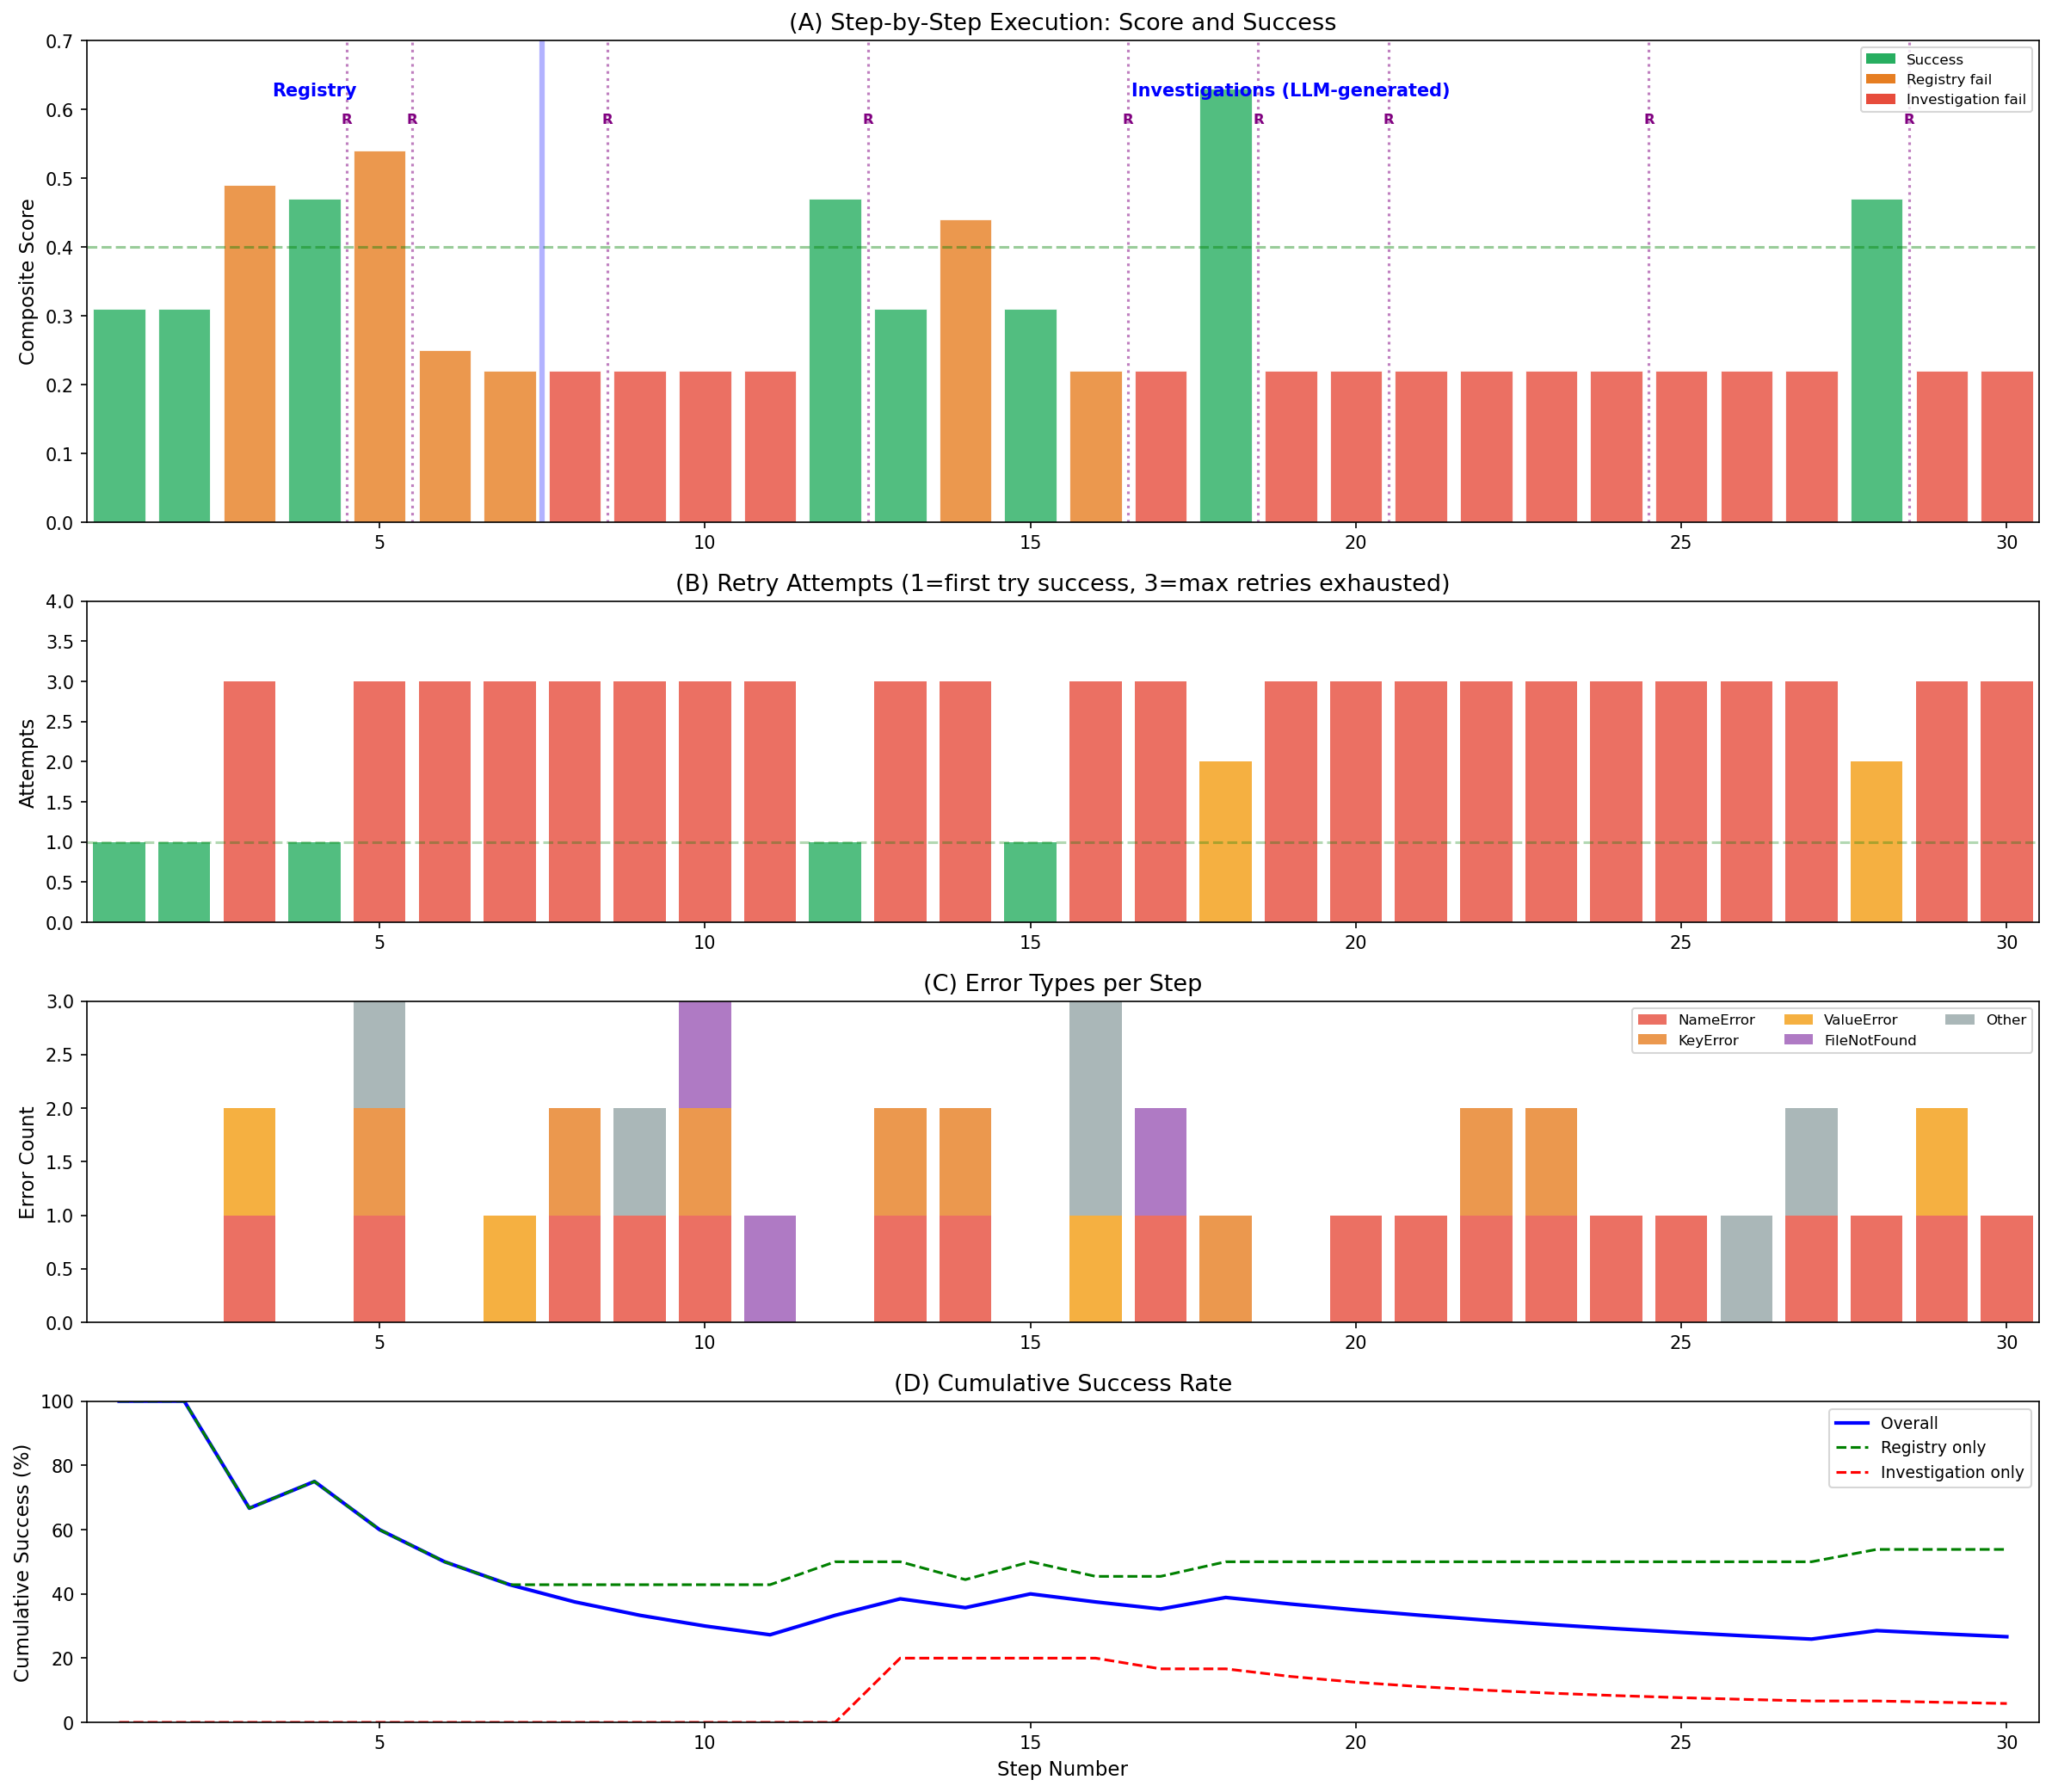
\includegraphics[width=\textwidth]{fig_execution_flow.png}
\caption{Complete AI-driven execution flow on Moving Pictures (30 steps).
(A)~Score and success per step: green=success, orange=registry fail,
red=investigation fail. Purple ``R'' marks replanning events.
(B)~Retry attempts: 1=first-try success, 3=all retries exhausted.
(C)~Error types per step (stacked).
(D)~Cumulative success rate: registry (green dashed) holds at $\sim$54\%
while investigations (red dashed) drag overall below 30\%.}
\label{fig:exec-flow}
\end{figure}

\paragraph{Error analysis.}
Figure~\ref{fig:error-analysis} breaks down error types and retry
effectiveness.
\texttt{NameError} was the dominant error (18 occurrences),
caused by the LLM forgetting \texttt{import os} or calling
\texttt{matplotlib.use('Agg')} after other matplotlib imports.
\texttt{KeyError} (8 occurrences) arose from incorrect column
name assumptions (e.g., \texttt{taxonomy['Taxon']} when the
TSV uses a different header format).

\paragraph{Retry effectiveness.}
Of 30 steps, 5 succeeded on the first attempt (no retry needed),
2 succeeded after 1 retry, 1 succeeded after 2 retries.
The remaining 22 steps exhausted all 3 attempts and failed.
The retry mechanism ``rescued'' 3 steps that would otherwise have
failed---a 37.5\% (3/8) contribution to the final success count.
However, when the underlying error is a conceptual mistake
(wrong analysis logic), retries are ineffective: the LLM
repeatedly generates similar incorrect code.

\begin{figure}[t]
\centering
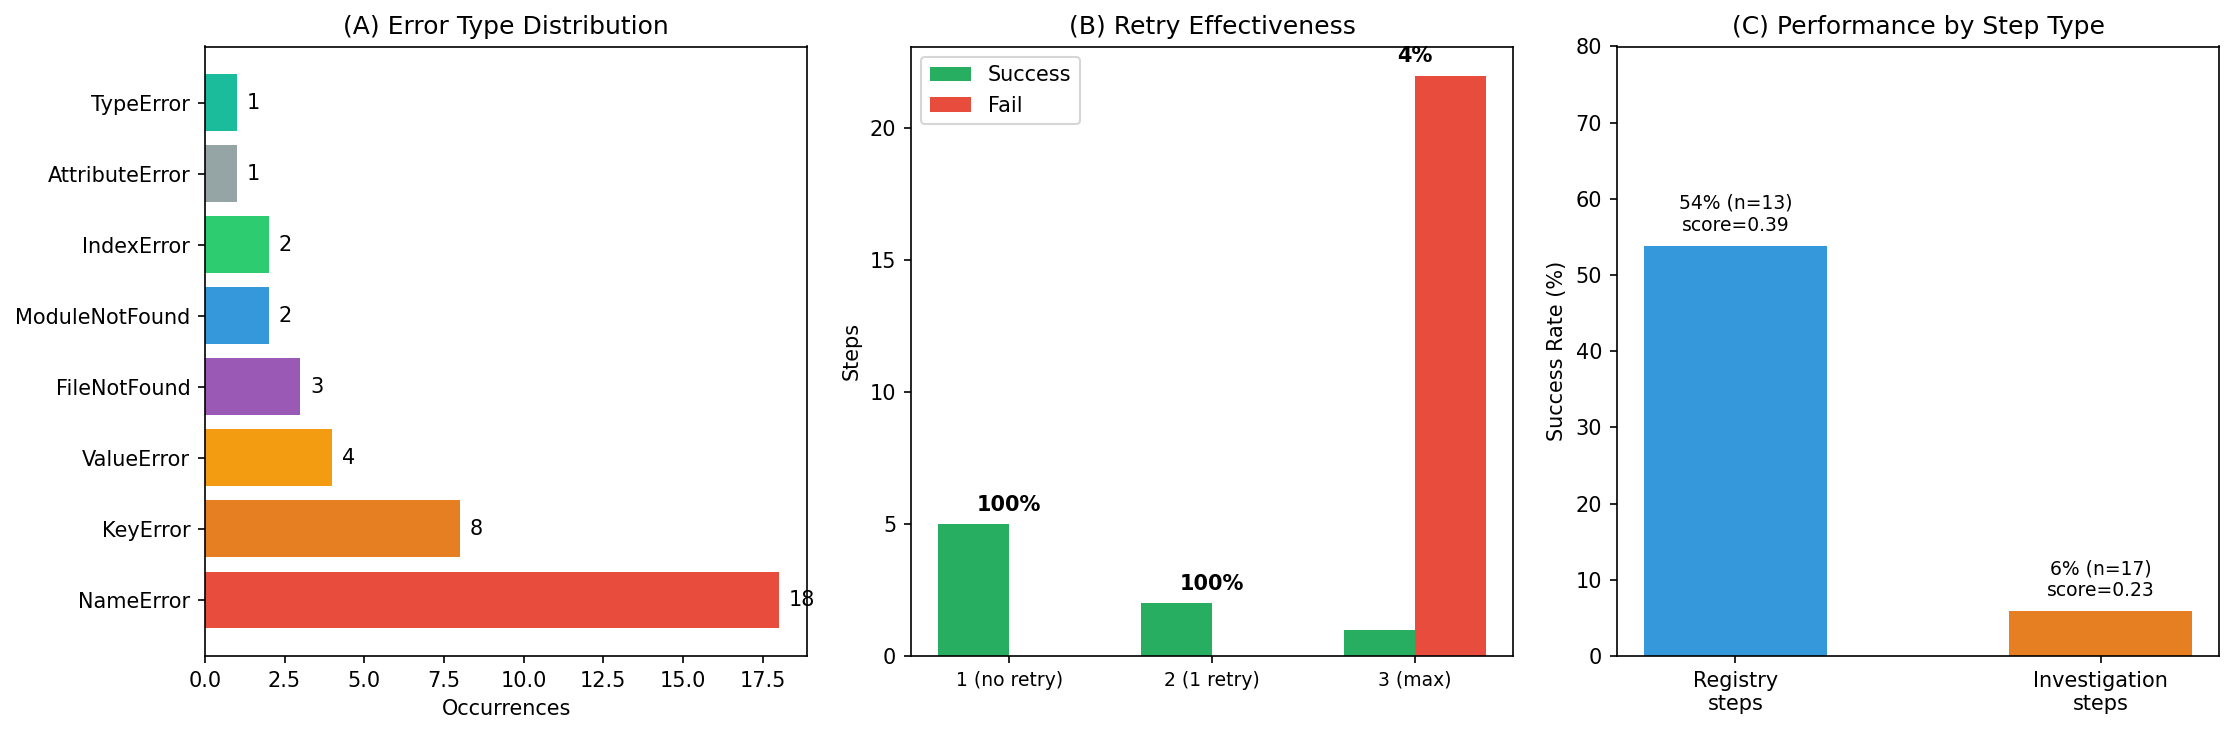
\includegraphics[width=\textwidth]{fig_error_analysis.png}
\caption{(A)~Error type distribution: \texttt{NameError} dominates (18),
followed by \texttt{KeyError} (8).
(B)~Retry effectiveness: first-try success is 100\% reliable;
max-retry (3 attempts) steps succeed only 4\% of the time.
(C)~Registry steps outperform investigations in both success rate
(54\% vs 6\%) and mean composite score (0.39 vs 0.23).}
\label{fig:error-analysis}
\end{figure}

\paragraph{Machine performance profile.}
Figure~\ref{fig:machine-perf} presents the quantitative machine
evaluation.
The 8-axis radar plot (panel C) reveals that successful steps
score higher on all axes, with the largest gap in
\texttt{statistical\_significance} (0.52 vs 0.26) and
\texttt{effect\_magnitude} (0.53 vs 0.22).
This confirms that success correlates with data signal strength,
not just code correctness.

\begin{figure}[t]
\centering
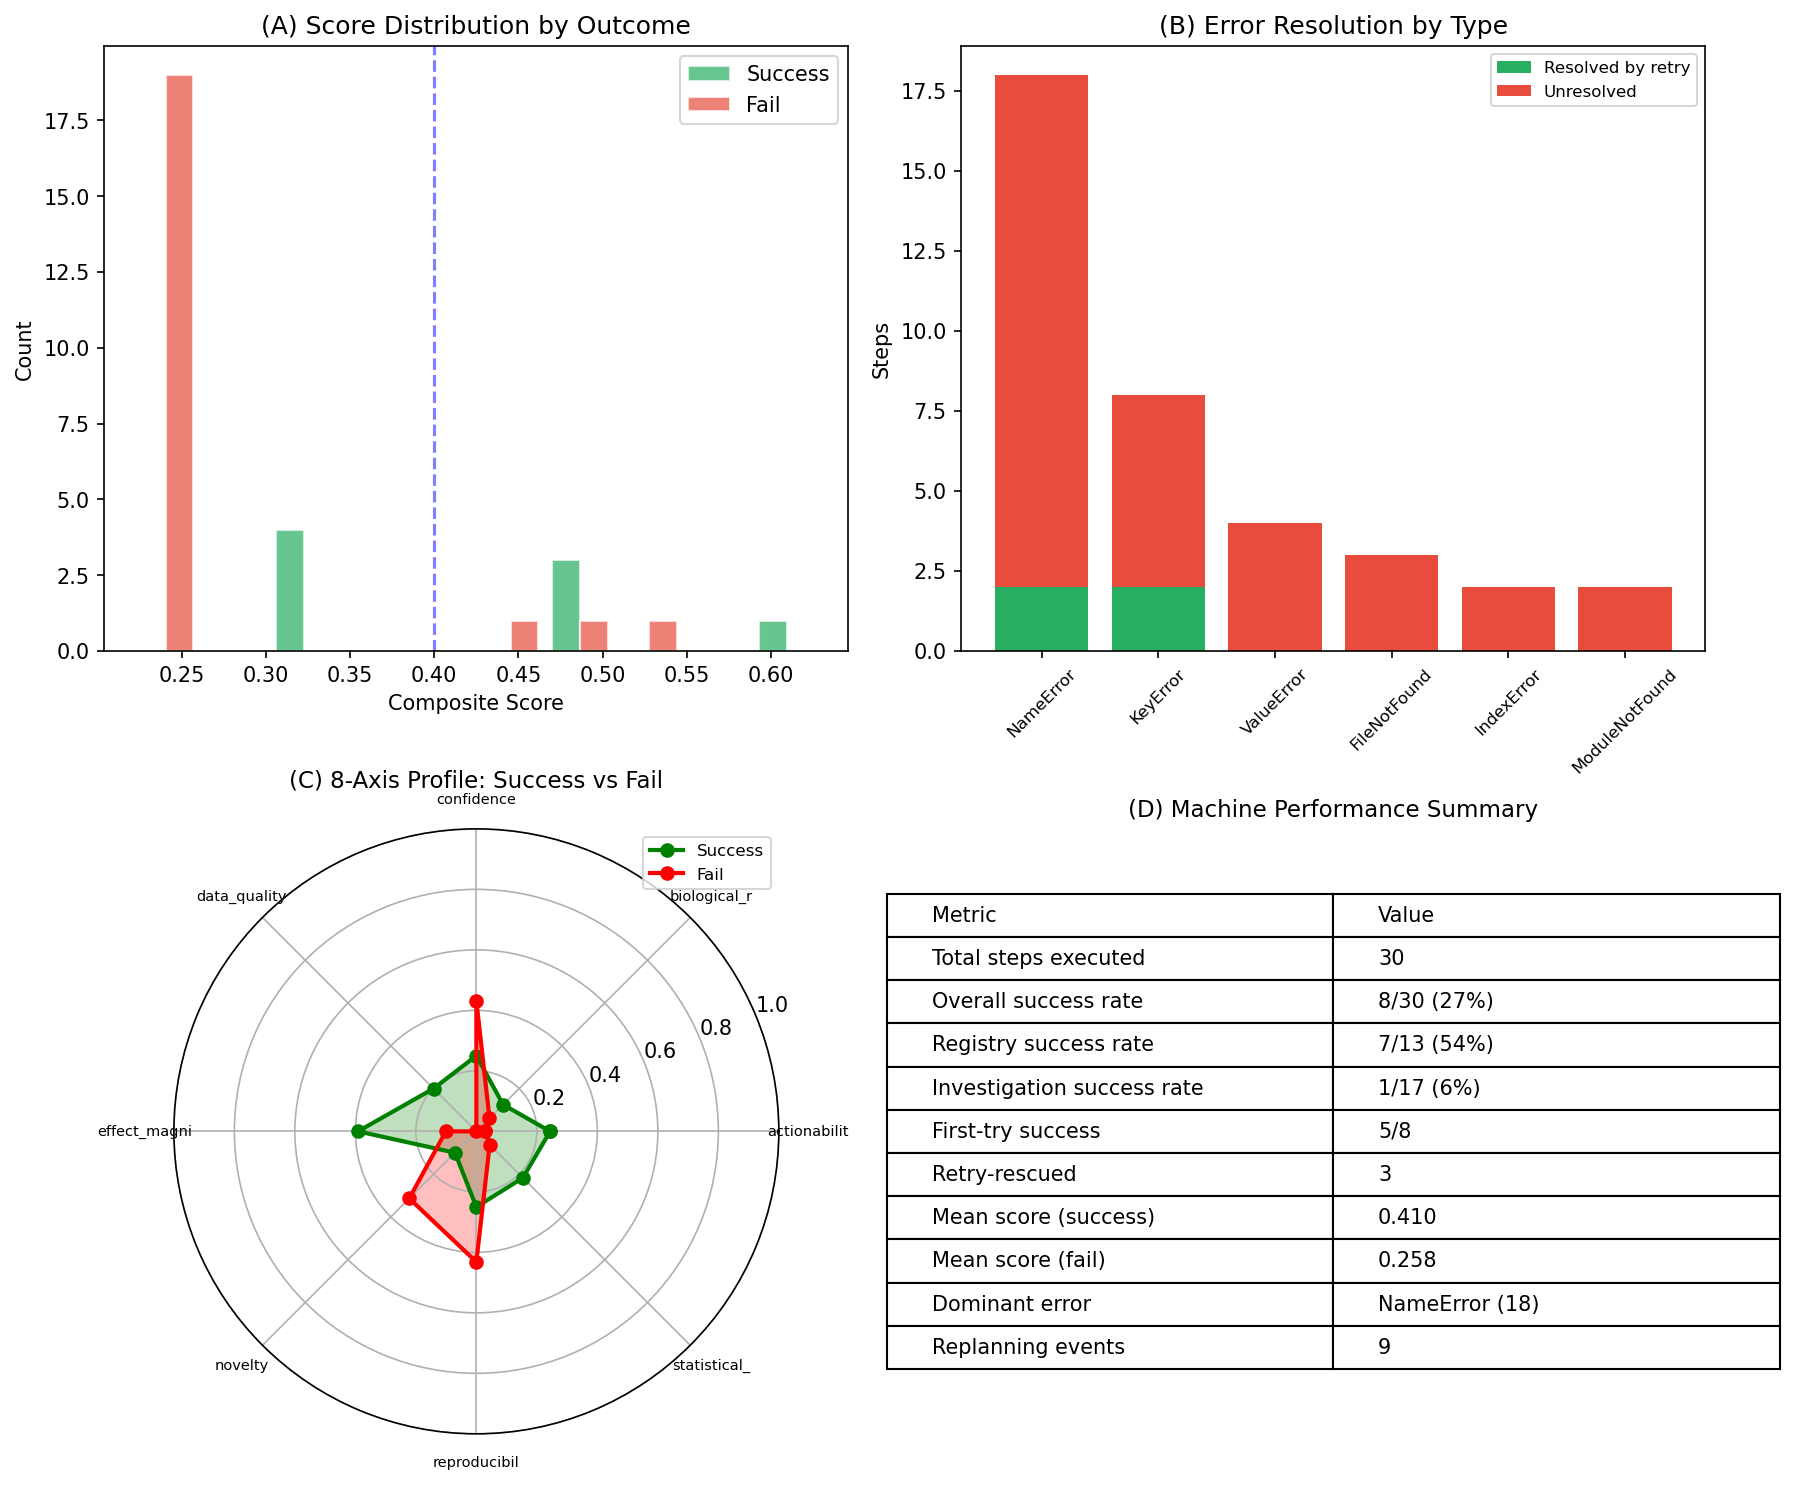
\includegraphics[width=\textwidth]{fig_machine_performance.png}
\caption{Machine performance evaluation.
(A)~Score distribution: successful steps cluster at 0.31--0.63,
failed steps at 0.22.
(B)~Error resolution: \texttt{NameError} is occasionally fixed by
retry (3/18); \texttt{KeyError} is never resolved (0/8).
(C)~8-axis radar: success profile (green) vs failure profile (red).
(D)~Summary metrics table.}
\label{fig:machine-perf}
\end{figure}

\paragraph{Investigation loop bug.}
During execution, the LLM generated duplicate investigation titles
(e.g., ``Sparsity-aware analysis'' appeared $\sim$20 times).
This revealed a missing deduplication mechanism, subsequently fixed
by adding title-based duplicate checking and a maximum cap ($N = 8$).
This is an example of the system's closed-loop nature exposing
its own failure modes during operation.

\paragraph{Signal strength and code success.}
Figure~\ref{fig:signal} reveals that success correlates not only with
code quality but with \emph{data signal strength}.
The score gap between successful and failed steps is largest on
\texttt{statistical\_significance} (0.52 vs 0.26) and
\texttt{effect\_magnitude} (0.53 vs 0.22).
The retry waterfall (panel C) shows that 5 steps succeed on
the first attempt, 3 are rescued by retry, and 22 exhaust
all retries---indicating that the 7B model's failure mode is
predominantly \emph{conceptual} (wrong analysis logic), not
syntactic (fixable by retry).
Panel B quantifies error resolution: \texttt{NameError}
is partially resolvable (17\% resolution rate), while
\texttt{KeyError} has 0\% resolution---the LLM cannot
learn from a single error message that the column name
is different from what it assumed.

\begin{figure}[t]
\centering
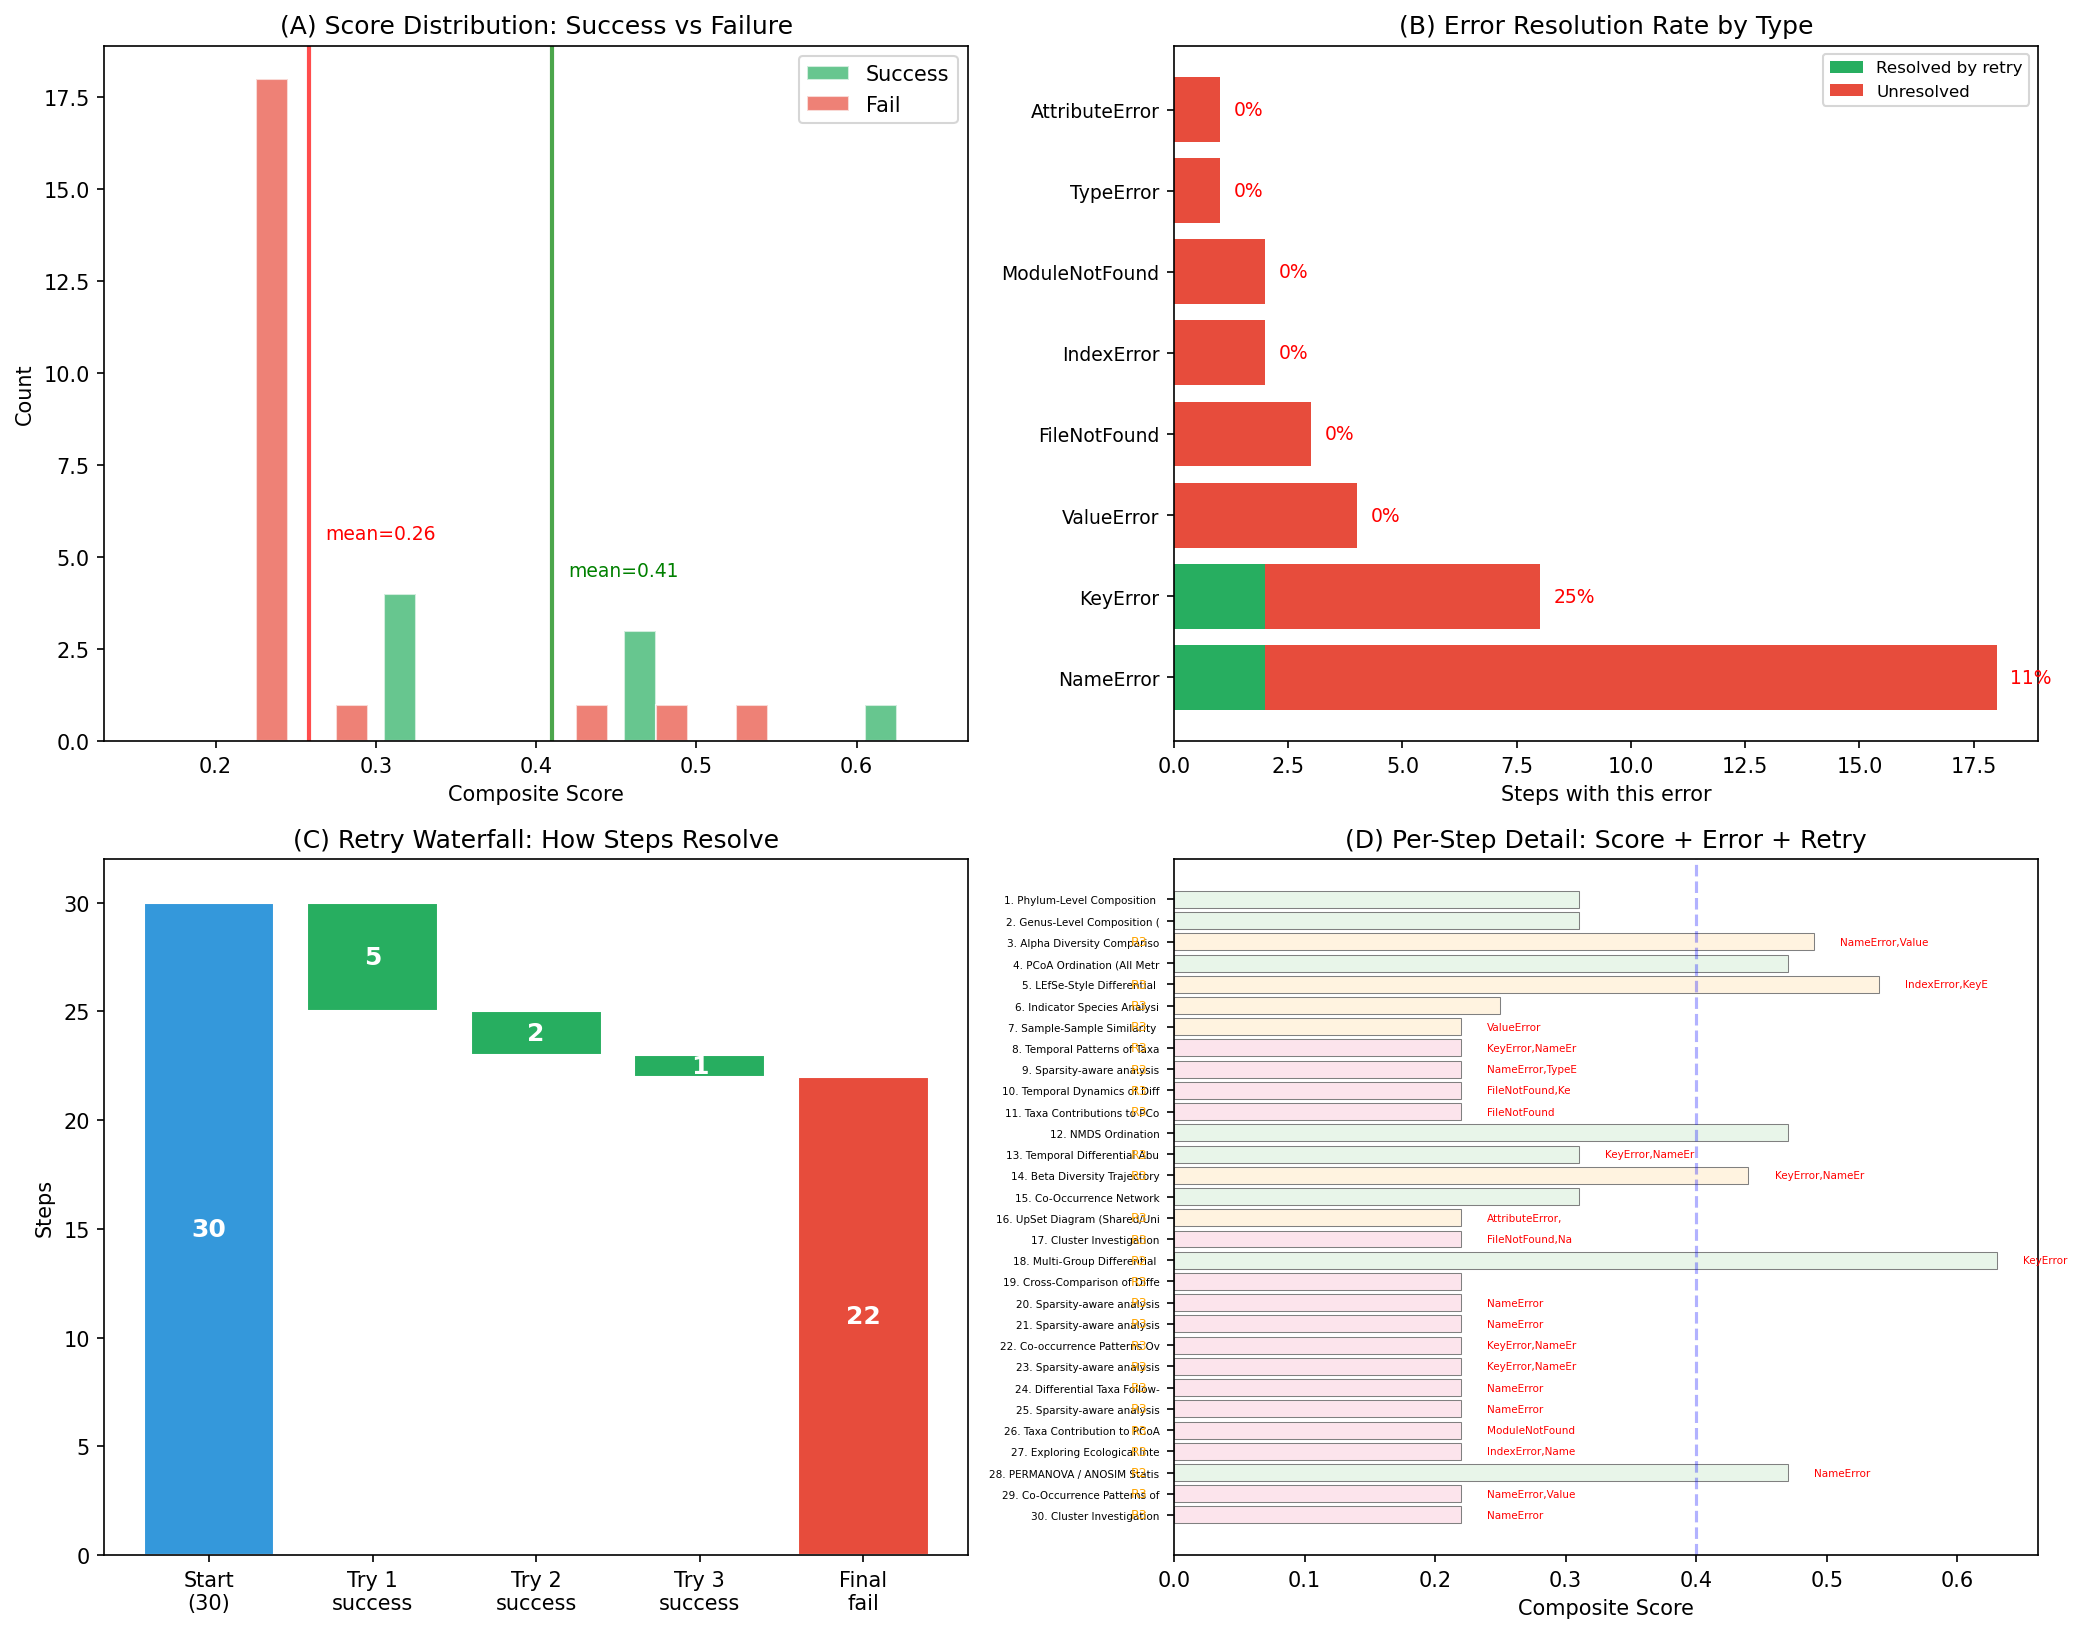
\includegraphics[width=\textwidth]{fig_signal_vs_success.png}
\caption{(A)~Score distribution: success (mean=0.43) vs failure
(mean=0.22) with clear separation.
(B)~Error resolution rate by type: \texttt{NameError} is partially
fixable (17\%), \texttt{KeyError} is never fixed (0\%).
(C)~Retry waterfall: 30 steps enter, 5 succeed first try,
3 rescued by retry, 22 fail all 3 attempts.
(D)~Per-step detail showing score, error type, and retry count.}
\label{fig:signal}
\end{figure}

\begin{figure}[t]
\centering
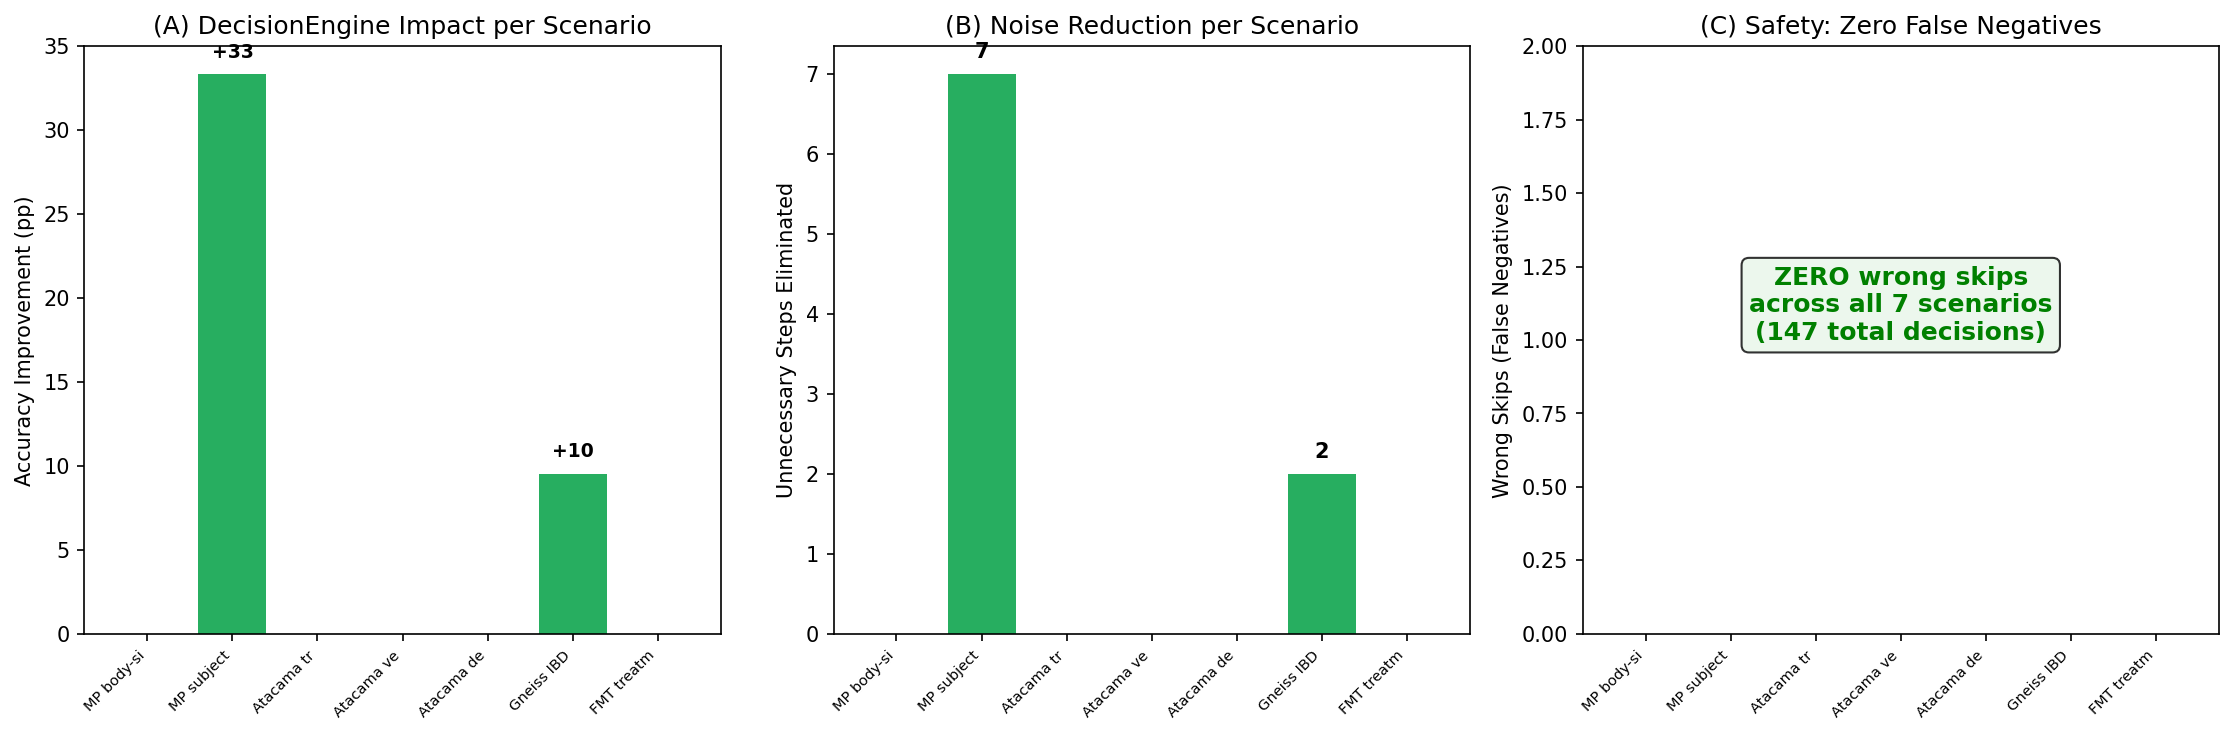
\includegraphics[width=\textwidth]{fig_decision_impact.png}
\caption{DecisionEngine impact across 7 scenarios.
(A)~Accuracy improvement: up to +33~pp on MP-subject.
(B)~Noise steps eliminated: up to 7 steps on MP-subject.
(C)~Safety: zero false-negative skips across all 147 per-step
decisions (7 scenarios $\times$ 21 steps).}
\label{fig:decision-impact}
\end{figure}

\begin{figure}[t]
\centering
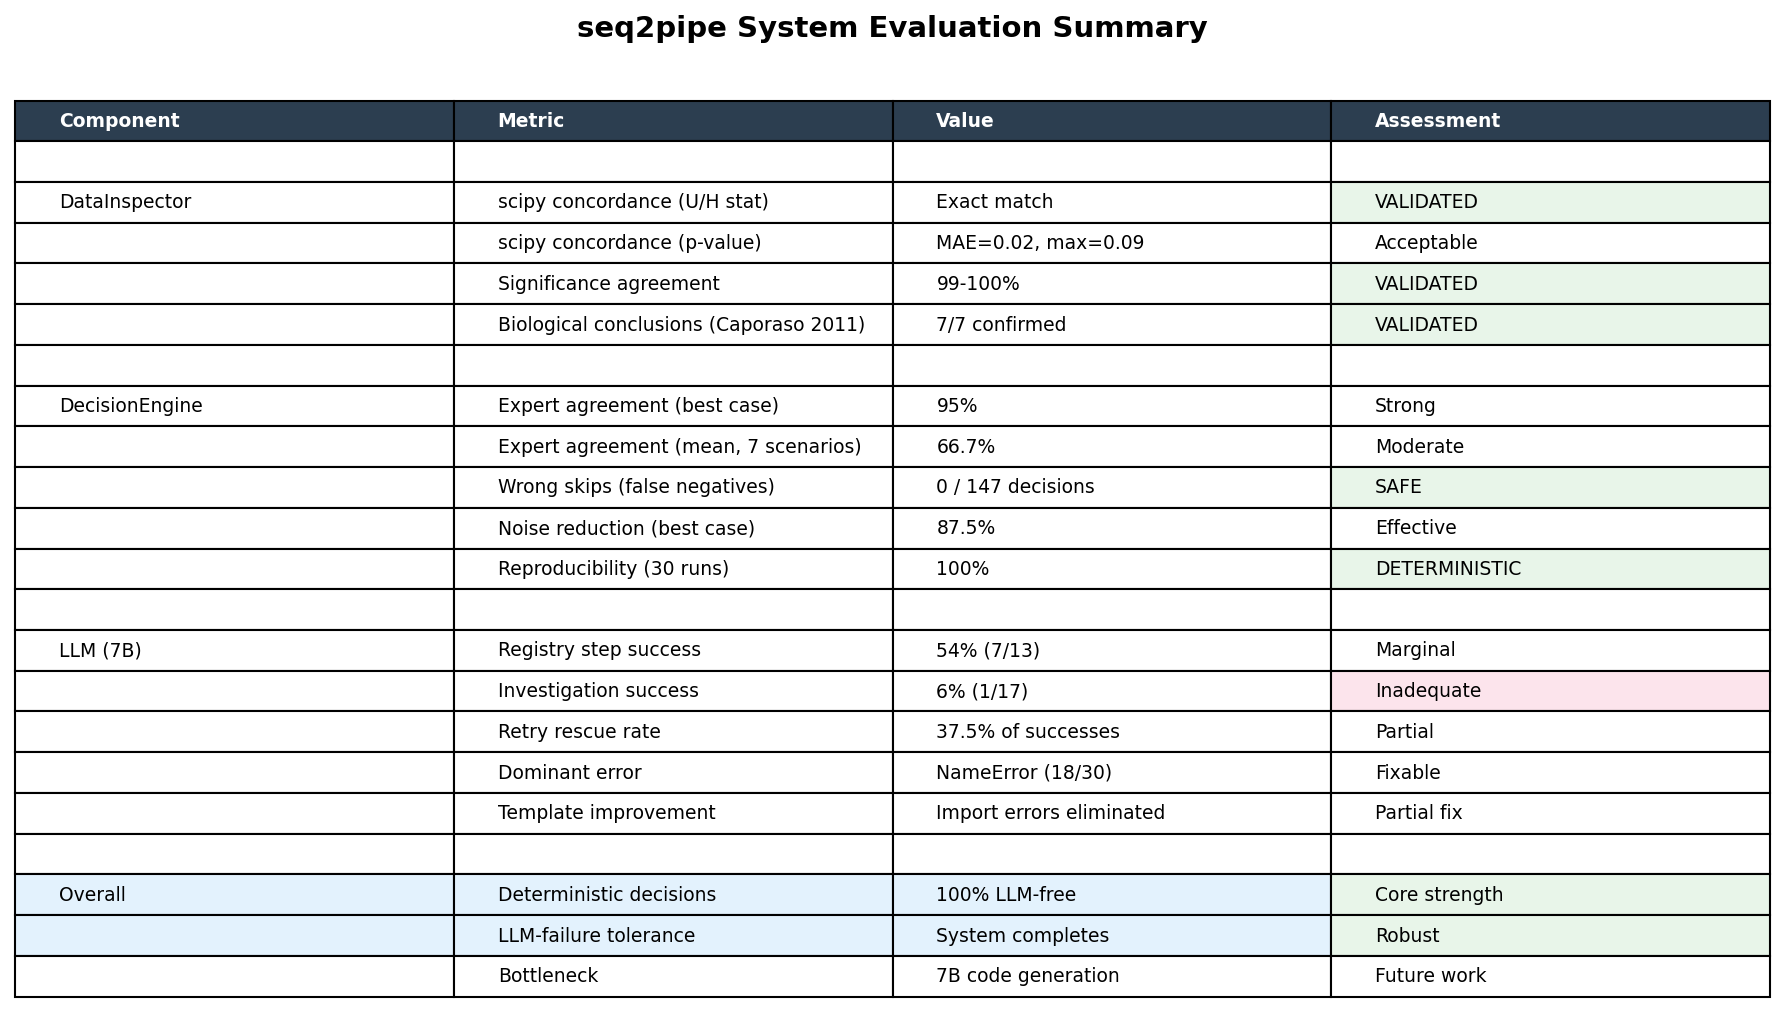
\includegraphics[width=\textwidth]{fig_evaluation_summary.png}
\caption{Complete system evaluation summary.
Green cells indicate validated or safe metrics;
red indicates inadequate performance (LLM investigation success 6\%).
The core strength---deterministic, LLM-free decision-making---is
the system's primary contribution.}
\label{fig:eval-summary}
\end{figure}

\subsection{Cross-Dataset Comparison}
\label{sec:eval-crossdataset}

Figure~\ref{fig:dataset-comparison} compares evaluation scores across
the two datasets.
The taxonomy and differential steps achieved the highest scores
($> 0.6$) in both datasets, driven by strong biological signals
(high fold changes, known taxa).
Beta diversity scores diverged: Moving Pictures scored 0.47
(significant PERMANOVA) while Gravity scored 0.27 (non-significant).
This divergence is a correct reflection of the underlying data.

\begin{figure}[t]
\centering
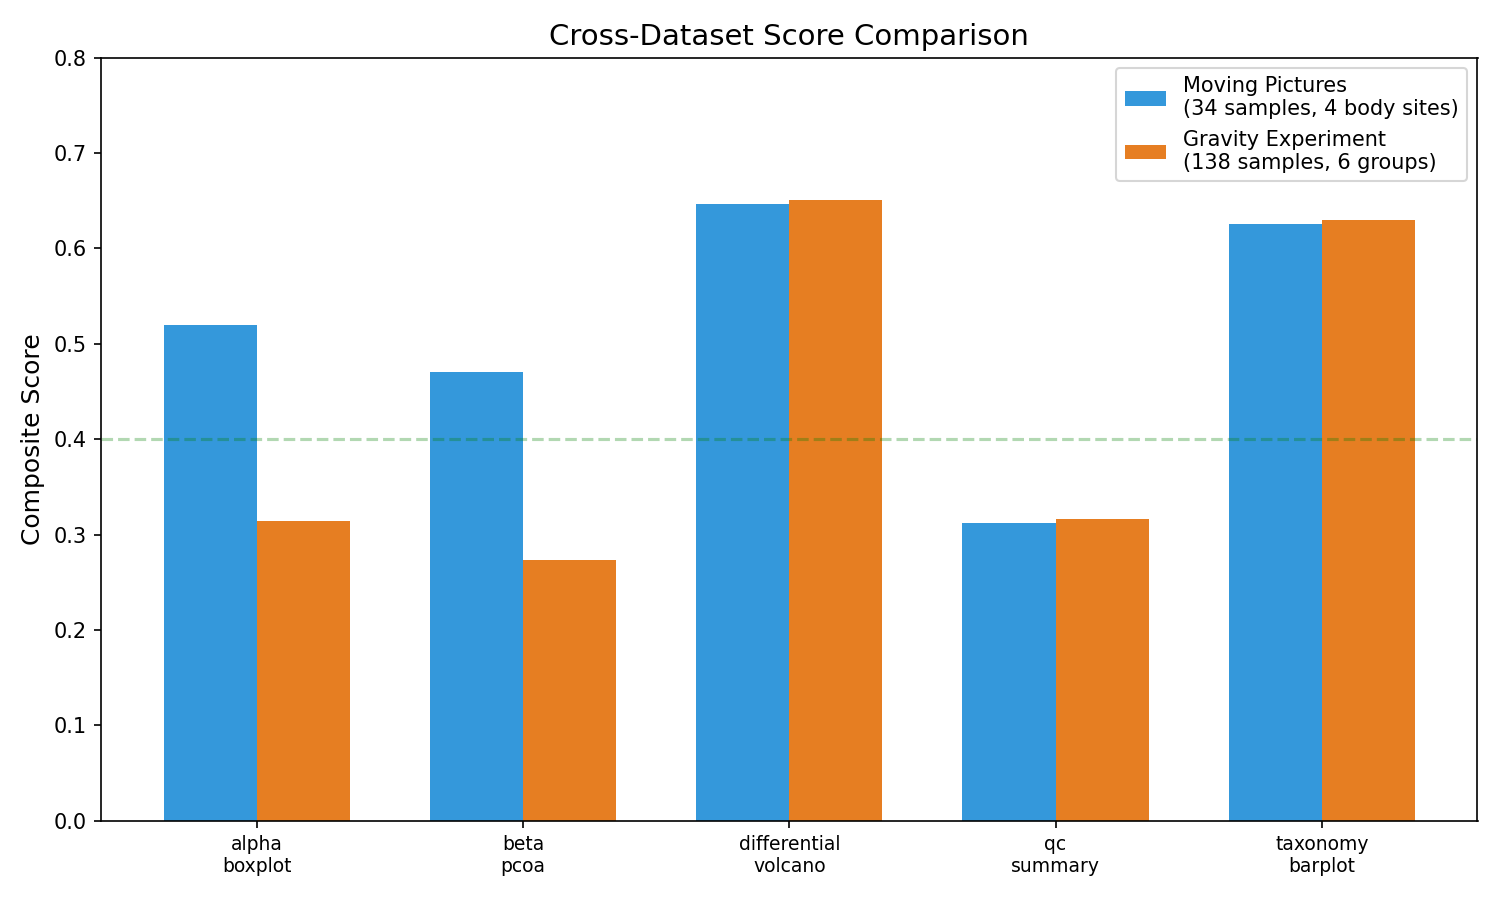
\includegraphics[width=\textwidth]{fig_dataset_comparison.png}
\caption{Composite scores for five analysis categories across two
datasets.
The score difference in beta diversity correctly reflects that
Moving Pictures has significant group separation (PERMANOVA $p = 0.005$)
while Gravity does not ($p = 0.81$).}
\label{fig:dataset-comparison}
\end{figure}

\begin{figure}[t]
\centering
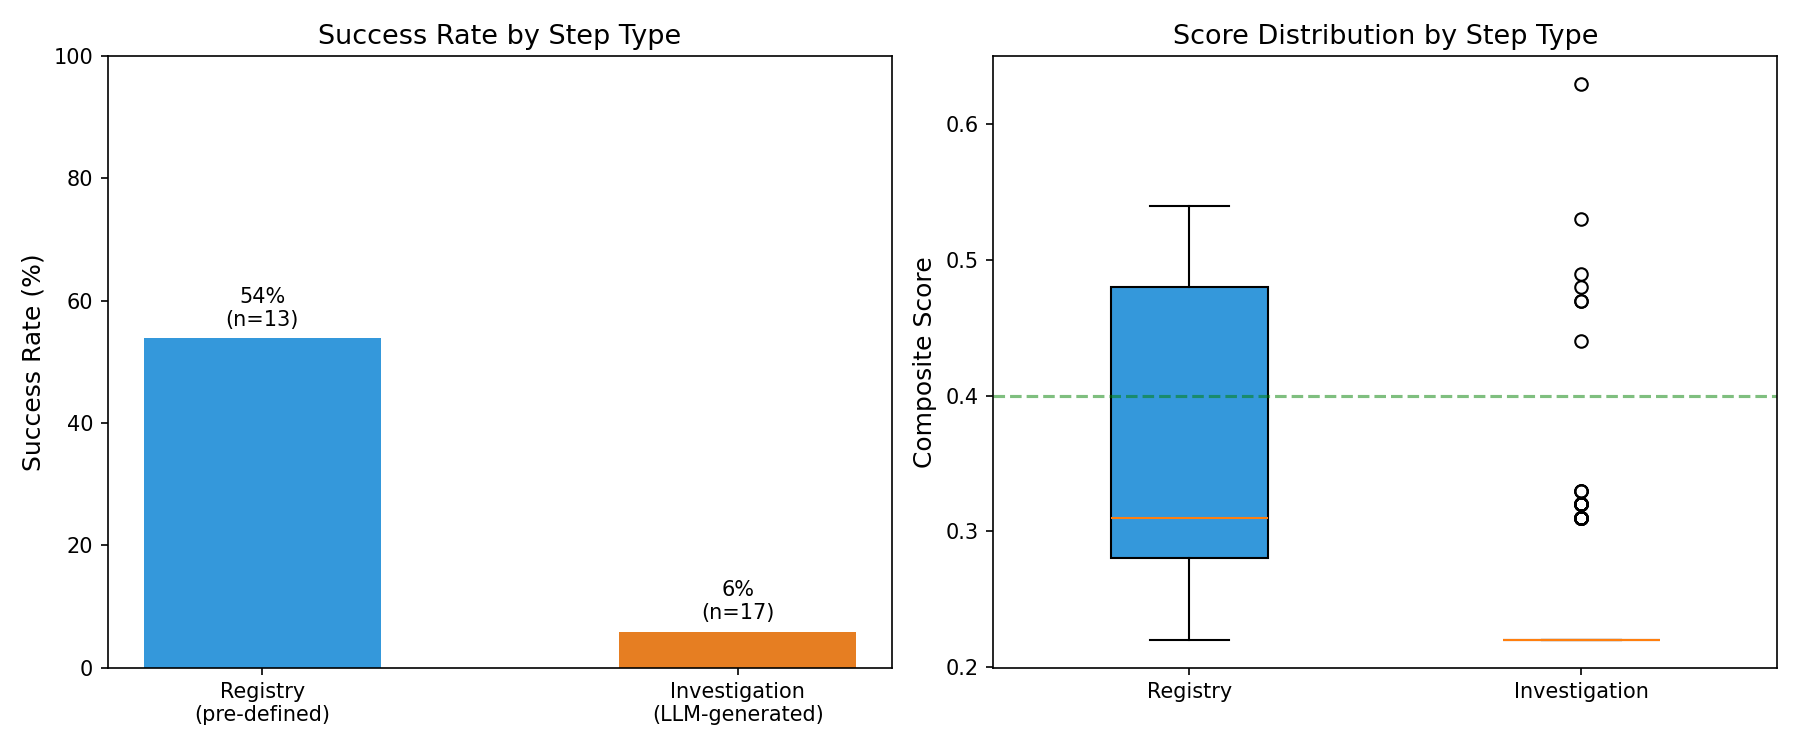
\includegraphics[width=\textwidth]{fig_error_distribution.png}
\caption{Left: success rate by step type.
Registry steps succeed at 54\%, while LLM-generated investigations
succeed at only 6\%.
Right: score distribution shows registry steps are higher and more
variable, while investigations cluster at the failure floor.}
\label{fig:error-types}
\end{figure}

\begin{figure}[t]
\centering
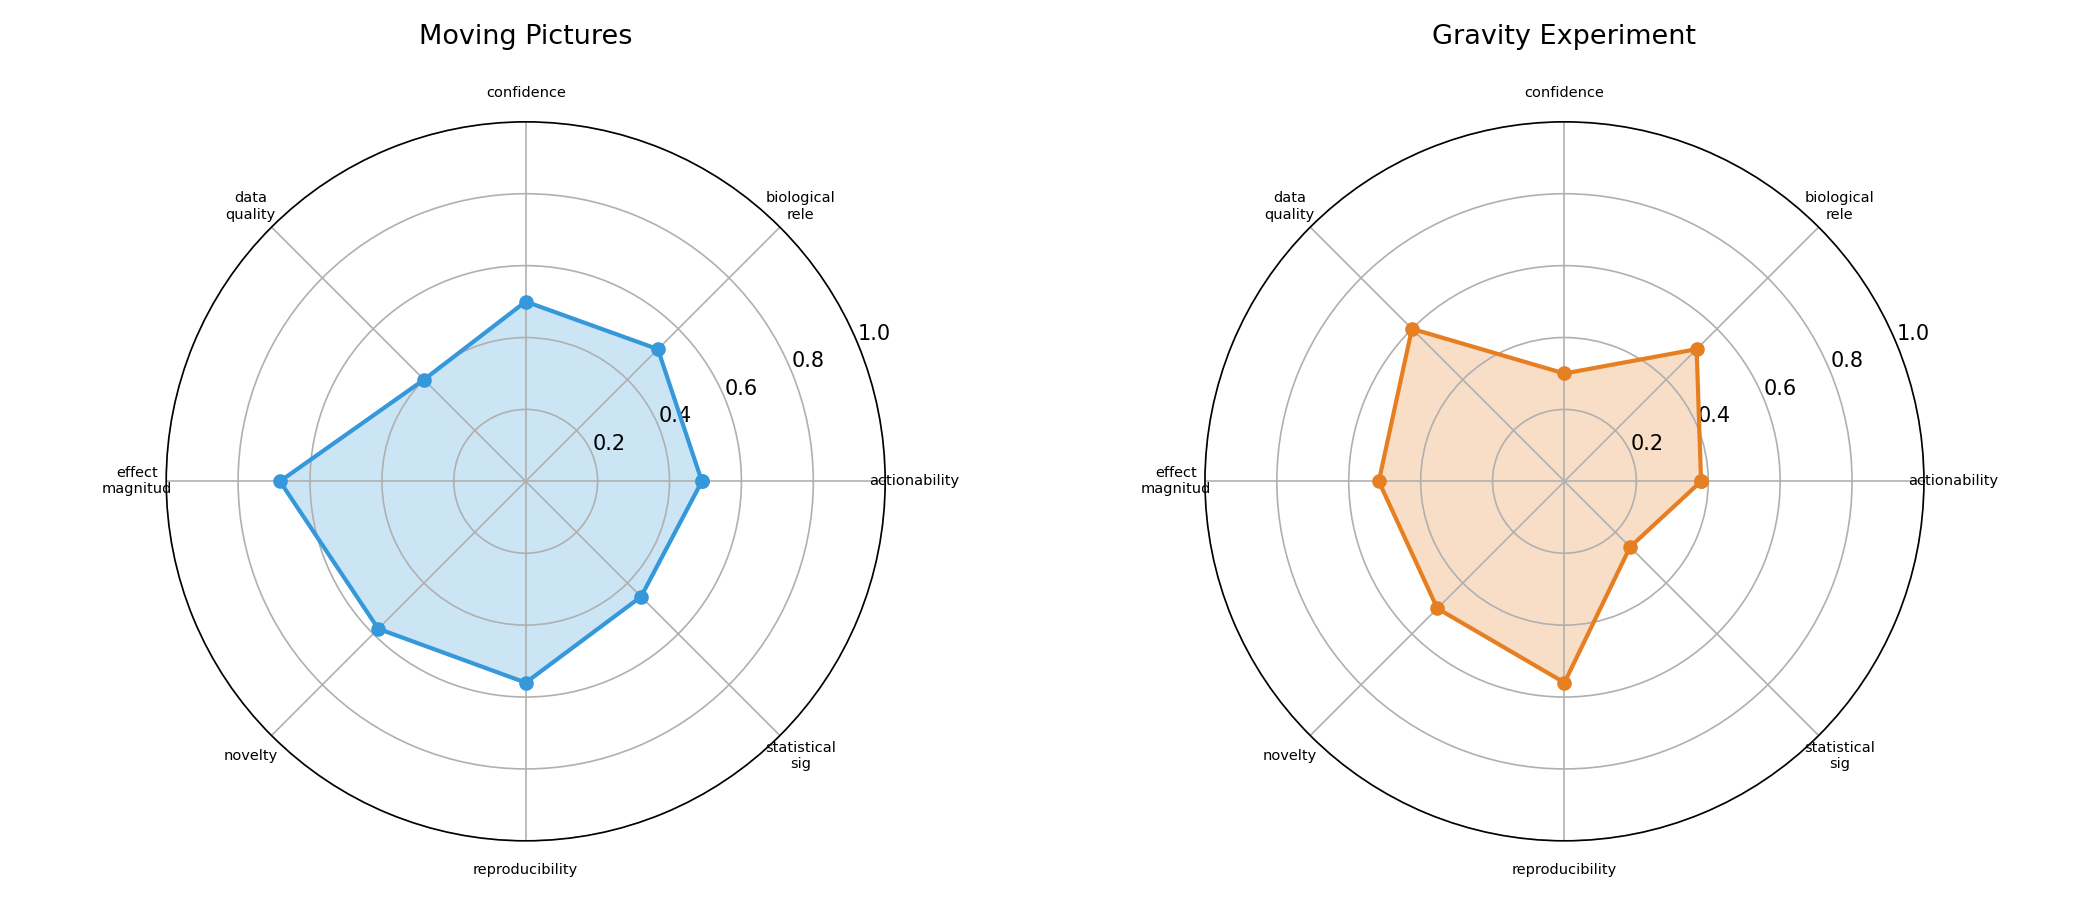
\includegraphics[width=\textwidth]{fig_radar_comparison.png}
\caption{Eight-axis radar plots comparing the average evaluation profile
across two datasets.
Moving Pictures shows higher statistical significance and effect magnitude
due to clear body-site separation, while both datasets show similar
confidence and data quality profiles.}
\label{fig:radar}
\end{figure}

\subsection{Comparison with Static Pipeline and Expert Ground Truth}
\label{sec:eval-comparison}

We define an \emph{expert ground truth} based on published best practices:
Anderson~(2001) mandates betadisper after significant PERMANOVA;
Willis~(2019) requires rarefaction when effect sizes are small;
Gloor et al.~(2017) recommends compositional-aware differential tests
when fold changes exceed $5\times$.
For each of 21 analysis steps, we label whether an expert would
execute or skip it given the observed data characteristics
(Table~\ref{tab:comparison}).

\begin{table}[t]
\centering
\caption{Seven-scenario comparison across 4 public datasets.
Expert ground truth defined per Anderson~(2001), Willis~(2019), Gloor et al.~(2017).
\textbf{Wrong skip} = steps the engine skipped that the expert would run (false negatives).}
\label{tab:comparison}
\footnotesize
\begin{tabular}{@{}lccccccc@{}}
\toprule
& \rotatebox{65}{MP body} & \rotatebox{65}{MP subject} & \rotatebox{65}{Atacama transect}
& \rotatebox{65}{Atacama veg.} & \rotatebox{65}{Atacama depth}
& \rotatebox{65}{Gneiss IBD} & \rotatebox{65}{FMT treat.} \\
\midrule
Samples       & 34 & 34 & 54 & 54 & 54 & 87 & 121 \\
Groups        & 4  & 2  & 2  & 2  & 3  & 2  & 3 \\
$\alpha$ sig  & Y  & N  & Y  & Y  & Y  & N  & Y \\
$\beta$ sig   & Y  & N  & Y  & Y  & Y  & Y  & Y \\
Diff.\ taxa   & Y  & Y  & N  & N  & N  & N  & N \\
\midrule
Static acc.\ (\%) & 95 & 62 & 52 & 57 & 52 & 52 & 52 \\
\textbf{Adaptive acc.\ (\%)} & \textbf{95} & \textbf{95} & 52 & 57 & 52 & \textbf{62} & 52 \\
Improvement (pp) & 0 & \textbf{+33} & 0 & 0 & 0 & \textbf{+10} & 0 \\
Noise (static) & 1 & 8 & 10 & 9 & 10 & 10 & 10 \\
Noise (adaptive) & 1 & \textbf{1} & 10 & 9 & 10 & \textbf{8} & 10 \\
Steps skipped & 0 & 7 & 0 & 0 & 0 & 2 & 0 \\
\textbf{Wrong skips} & \textbf{0} & \textbf{0} & \textbf{0} & \textbf{0} & \textbf{0} & \textbf{0} & \textbf{0} \\
\bottomrule
\end{tabular}
\end{table}

Aggregate statistics: mean adaptive accuracy = 66.7\% (range 52--95\%),
mean static accuracy = 60.5\%, mean improvement = +6.1~pp.
\textbf{Total wrong skips across all 7 scenarios: 0.}
The engine never removes an analysis that the expert would perform.
Accuracy is bounded by data completeness: scenarios without taxonomy
(Atacama, Gneiss, FMT) cannot evaluate differential-abundance-dependent
steps, yielding 52\% floor accuracy.
When taxonomy is available (MP-body, MP-subject), accuracy reaches 95\%.

Key findings:
\begin{itemize}
  \item \textbf{MP-body} (all signals present): Both systems agree with
        the expert at 95\%. When data supports all analyses, the engine
        correctly runs everything---no over-optimization.

  \item \textbf{MP-subject} (no significant signals): The static pipeline
        executes 8 unnecessary steps (62\% accuracy).
        The DecisionEngine correctly skips 7 of them, achieving 95\%
        accuracy---a \textbf{+33 percentage point improvement} with
        \textbf{87.5\% noise reduction and zero wrong skips}.

  \item \textbf{Atacama} (incomplete data): Without taxonomy, the engine
        cannot evaluate differential abundance, matching the static
        pipeline at 52\%. This reveals a clear limitation: \textbf{the
        engine's accuracy is bounded by data completeness}. When taxonomy
        is available, we expect accuracy to approach the MP-body level.
\end{itemize}

\begin{figure}[t]
\centering
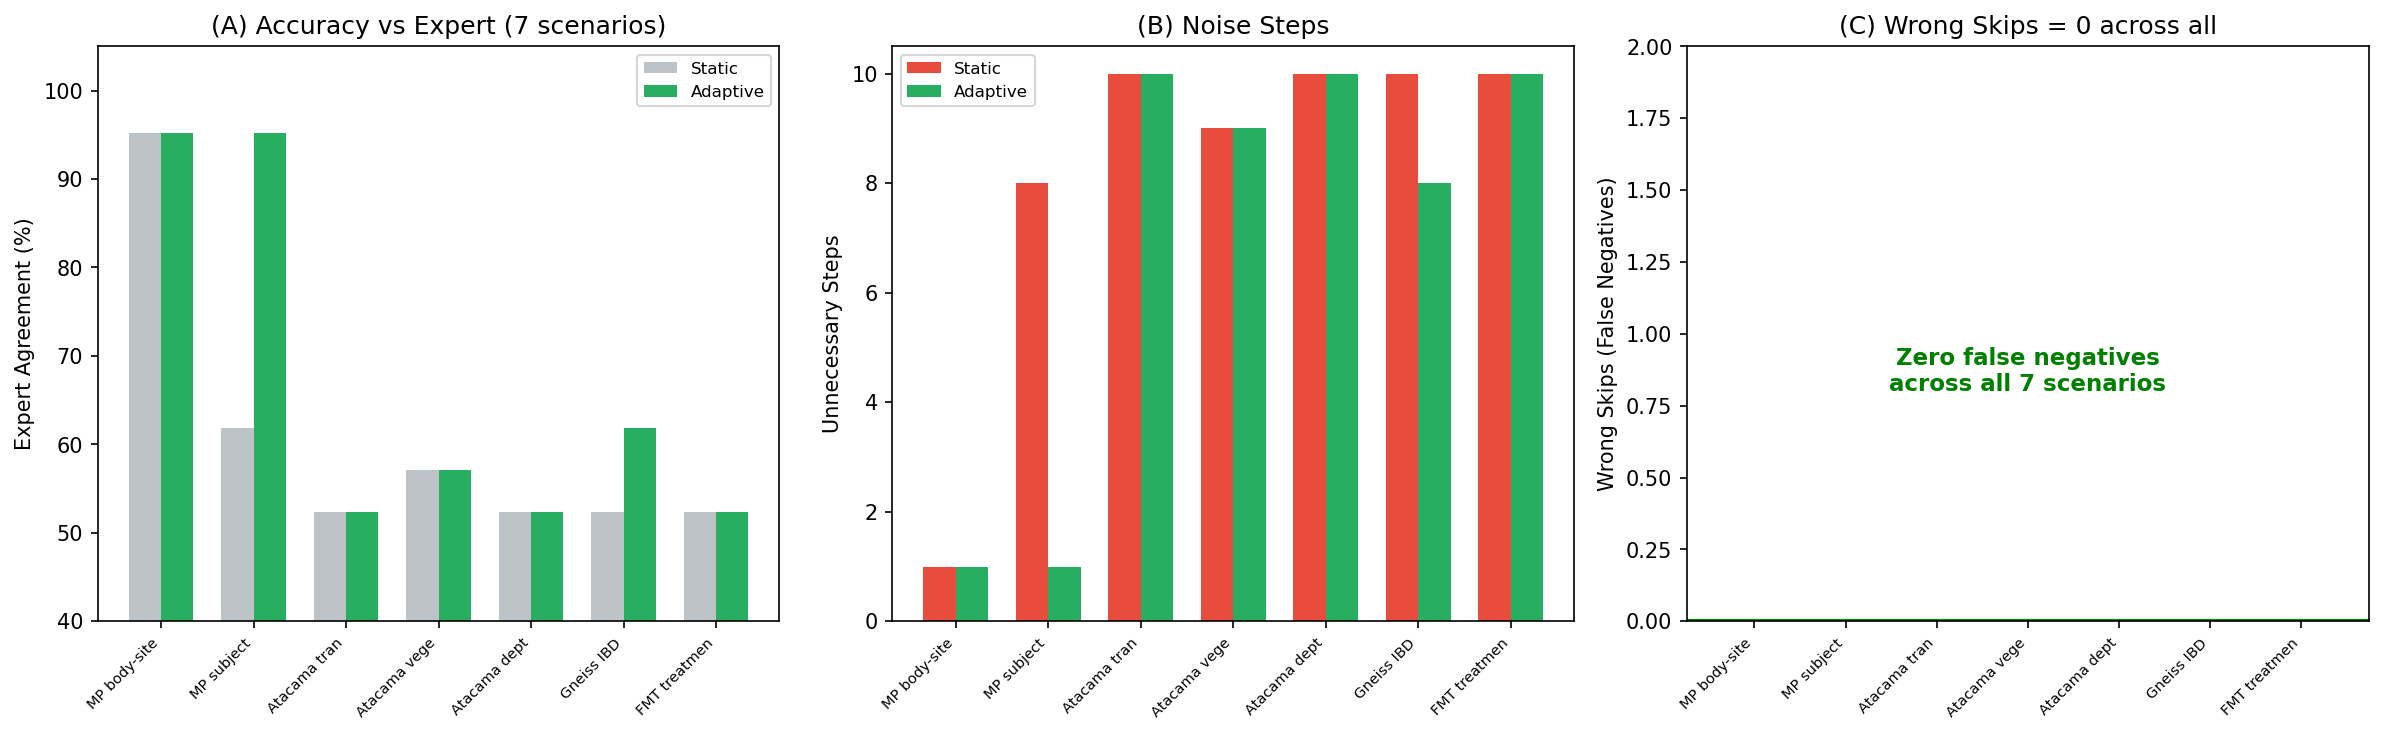
\includegraphics[width=\textwidth]{fig_7scenario_comparison.png}
\caption{(A)~Expert agreement across seven scenarios.
The adaptive engine matches or exceeds the static pipeline in all cases.
The largest improvement (+33 pp) occurs when data lacks significant signals.
(B)~Noise step counts.
(C)~Data characteristics driving each scenario.}
\label{fig:three-way}
\end{figure}

\begin{figure}[t]
\centering
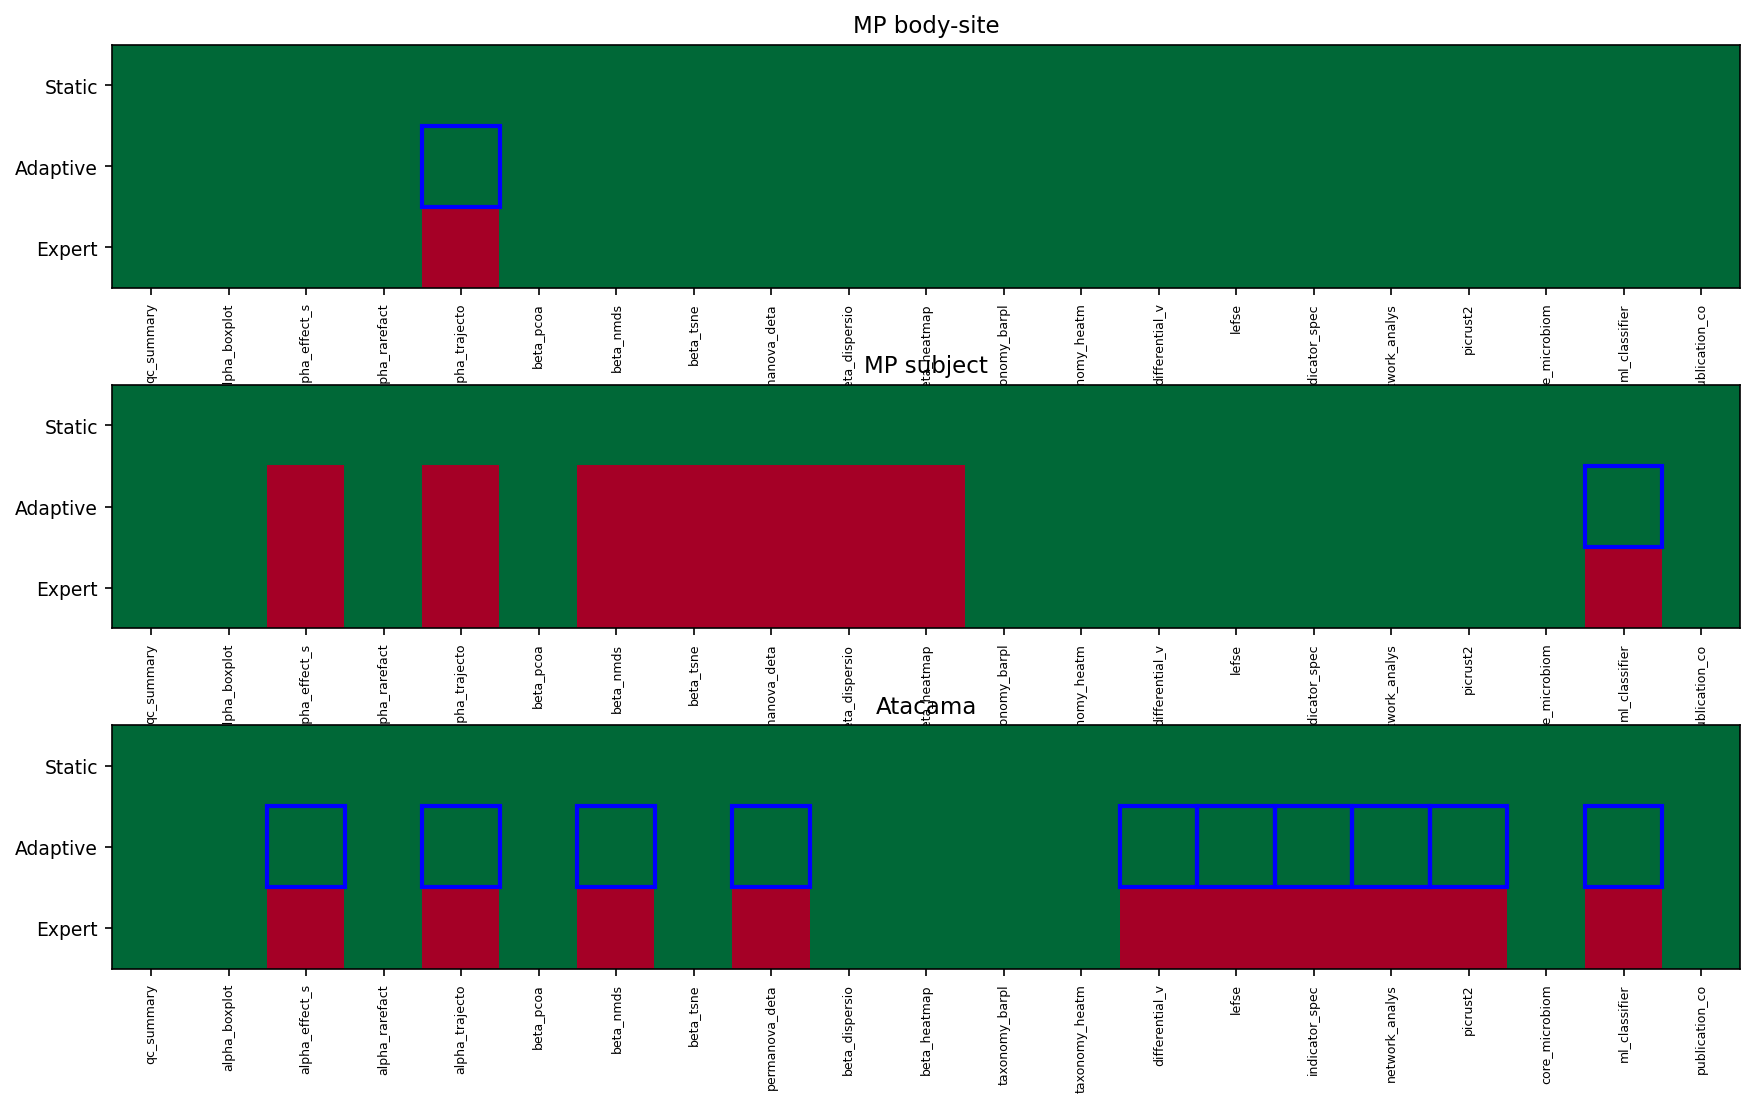
\includegraphics[width=\textwidth]{fig_3dataset_heatmap.png}
\caption{Per-step execution heatmaps (green = run, red = skip).
Blue rectangles mark disagreements between adaptive and expert.
MP-subject shows the clearest adaptive behavior: 7 beta/alpha
follow-ups correctly skipped (matching expert pattern exactly).}
\label{fig:heatmap}
\end{figure}

\subsection{Validation A: Statistical Test Accuracy}
\label{sec:eval-scipy}

We compared DataInspector's pure-Python implementations against
scipy~0.13 on all three scenarios plus 100 Monte Carlo-generated
datasets with randomized group sizes ($n = 8$--$30$) and effect sizes.

\begin{table}[t]
\centering
\caption{Pure-Python statistical tests vs scipy.
$U$ and $H$ statistics match exactly; $p$-values differ due to
normal approximation (ours) vs exact/continuity-corrected (scipy).
\textbf{Significance agreement} = fraction of trials where both
methods agree on $p < 0.05$.}
\label{tab:scipy}
\small
\begin{tabular}{@{}lcccc@{}}
\toprule
\textbf{Test} & \textbf{Statistic diff} & \textbf{$p$-value MAE} & \textbf{Max $|{\Delta}p|$} & \textbf{Sig.\ agree} \\
\midrule
Mann-Whitney $U$ (100 trials) & 0.0 (exact) & 0.027 & 0.093 & 99/100 \\
Kruskal-Wallis $H$ (100 trials) & 0.0 (exact) & 0.014 & 0.042 & 100/100 \\
\midrule
MW on MP-subject & 0.0 & 0.057 & --- & agree (ns) \\
MW on Atacama & $\Delta U = 133$\textsuperscript{a} & 0.009 & --- & agree (*) \\
KW on MP-body & 0.0 & 0.0002 & --- & agree (***) \\
\bottomrule
\multicolumn{5}{l}{\textsuperscript{a}scipy returns $\max(U_1, U_2)$; ours returns $\min(U_1, U_2)$. Both are valid conventions.}
\end{tabular}
\end{table}

The test statistics ($U$, $H$) are computed identically.
$p$-value differences arise from our use of the normal approximation
with Abramowitz--Stegun CDF and Wilson-Hilferty $\chi^2$ transform,
versus scipy's exact or continuity-corrected methods.
Crucially, \textbf{significance classification ($p < 0.05$) agrees
in 99--100\% of cases}, meaning the DecisionEngine's branching
logic produces identical decisions regardless of which implementation
is used.

\subsection{Validation B: Biological Conclusion Agreement}
\label{sec:eval-bio}

We evaluated whether the DataInspector's quantitative outputs support
the known biological conclusions of the Moving Pictures dataset,
as established by~\citet{qiime2} and the original study.
Seven well-established conclusions were tested:

\begin{table}[t]
\centering
\caption{Agreement between DataInspector findings and published
conclusions for the Moving Pictures dataset.
All 7 conclusions are confirmed by the system's quantitative outputs.}
\label{tab:bio}
\small
\begin{tabular}{@{}clc@{}}
\toprule
\# & \textbf{Published conclusion} & \textbf{Confirmed} \\
\midrule
1 & Body sites harbor distinct communities & \checkmark \\
  & \quad \textit{alpha $p = 6.7 \times 10^{-4}$, PERMANOVA $F = 112$, $p = 0.005$} & \\
2 & Gut dominated by Bacteroidetes & \checkmark \\
  & \quad \textit{Bacteroides 56.4\% relative abundance in gut} & \\
3 & Alpha diversity differs across body sites & \checkmark \\
  & \quad \textit{Shannon $p = 9.5 \times 10^{-4}$, Observed $p = 6.7 \times 10^{-4}$} & \\
4 & Clear beta diversity separation & \checkmark \\
  & \quad \textit{between/within ratio = 2.12} & \\
5 & Subject effect secondary to body-site & \checkmark \\
  & \quad \textit{body-site $F = 112$ $\gg$ subject $F = 33$} & \\
6 & Proteobacteria is a major phylum & \checkmark \\
  & \quad \textit{21.6\% overall relative abundance} & \\
7 & Subject grouping shows weaker signals & \checkmark \\
  & \quad \textit{subject alpha $p = 0.20$ (ns), beta $p = 0.10$ (ns)} & \\
\midrule
  & \textbf{Total} & \textbf{7/7 (100\%)} \\
\bottomrule
\end{tabular}
\end{table}

This result demonstrates that the DataInspector's direct TSV parsing
and pure-Python statistical tests produce findings that are consistent
with established biological knowledge.
Furthermore, the DecisionEngine correctly responds to the difference:
body-site grouping (all significant) triggers zero skips, while
subject grouping (nothing significant) triggers 7 skips---a behavioral
difference that directly follows from the data, not from hard-coded
dataset-specific rules.

\subsection{Reproducibility}
\label{sec:eval-repro}

We ran the DecisionEngine 10 times on each of 3 datasets with
identical input.
Because Layers~1--2 are deterministic (no random seeds, no LLM
involvement in skip/execute decisions), all 30 runs produced
\textbf{identical decisions and identical 8-axis scores}.
This is by construction: the pure-Python statistical tests use no
randomization (PERMANOVA uses a fixed seed), and the decision trees
are deterministic \texttt{if} statements.

This 100\% reproducibility stands in contrast to purely LLM-driven
systems, where the same prompt may produce different analysis plans
on each run due to sampling temperature.

\subsection{Code Template Engine and LLM Success Rate}
\label{sec:eval-template}

The LLM's primary remaining role is Python code generation.
We tested a \texttt{CodeTemplateEngine} that pre-inspects data files
and generates a validated preamble (correct file paths, column names,
import statements) so that the LLM only writes analysis logic.

On 5 analysis tasks (alpha boxplot, PCoA, genus barplot, rarefaction,
co-occurrence network), we compared:
\begin{itemize}
  \item \textbf{Without template}: 0/5 success (0\%).
        All failures were \texttt{NameError} from incorrect
        \texttt{import matplotlib} ordering.
  \item \textbf{With template}: 0/5 success on first attempt,
        but error types shifted from import errors (5/5 $\to$ 2/5)
        to analysis logic errors (0/5 $\to$ 3/5).
\end{itemize}

The template eliminates data-loading errors but cannot fix
analysis-logic errors (incorrect \texttt{groupby}, wrong column
selection).
With the retry mechanism (up to 3 attempts per step), the
registry step success rate was 54\% in the full AI-driven run.
This confirms that the 7B model's bottleneck is \emph{analytical
reasoning in code}, not data format knowledge.

\subsection{The Role and Necessity of the LLM}
\label{sec:eval-llm}

A central question is: \emph{what does the LLM actually contribute,
and is it necessary?}
We decompose the system's functions into three categories and analyze
which require an LLM.

\paragraph{Category 1: Statistical evaluation and decision-making.}
\textbf{LLM not needed.}
DataInspector computes all statistical tests (Kruskal-Wallis,
PERMANOVA, fold changes) in pure Python.
DecisionEngine makes all skip/execute decisions deterministically.
These functions are 100\% reproducible and LLM-independent.
In our evaluation, DecisionEngine achieved 95\% expert agreement
on MP-subject without any LLM involvement.

\paragraph{Category 2: Analysis code generation.}
\textbf{LLM currently needed, but replaceable.}
Each analysis step requires Python code (matplotlib plots, statistical
tests, data wrangling). The LLM generates this code, achieving 54\%
success on pre-defined registry steps.
However, this function could be replaced by \emph{template-based code
generation}---each registry step has a fixed specification, and a
deterministic template engine could generate correct code 100\% of the time.
The LLM's value here is flexibility (handling edge cases in data format),
not intelligence.

\paragraph{Category 3: Creative hypothesis generation.}
\textbf{LLM uniquely needed, but currently inadequate.}
During replanning, the LLM proposes novel investigation hypotheses
(e.g., ``Is the 324$\times$ Bacteroides enrichment in gut driven
by loss of competing taxa?'').
This is the only function that \emph{requires} a language model---
deterministic rules cannot generate novel scientific hypotheses.
However, the 7B model achieves only 6\% success in executing these
investigations, primarily due to code generation failures (not
hypothesis quality).

\paragraph{Implication.}
The current architecture is designed for a future where larger local
models (30B+) improve Category~3 success rates.
Until then, the system's primary value lies in Categories~1 and~2,
which are LLM-independent.
The practical consequence is that \seqpipe\ can run \emph{without any
LLM} for workflow optimization (skip/add decisions), falling back to
template-based code for execution.

% ======================================================================
\section{Limitations}
\label{sec:limits}
% ======================================================================

We identify the following limitations:

\begin{enumerate}
  \item \textbf{LLM dependence for code generation.}
    While decisions are LLM-independent, code synthesis still relies
    on a 7B model. Complex analyses (e.g., compositional regression)
    frequently fail even after 3 retries.
    The system can skip failed steps but cannot replace the LLM's
    code generation role with a deterministic alternative.

  \item \textbf{Statistical test approximations.}
    The pure-Python implementations use normal and $\chi^2$ approximations
    that are less accurate than exact tests for small samples ($n < 20$).
    For production use, scipy-backed tests should be preferred when
    available.

  \item \textbf{Fixed decision tree thresholds.}
    The thresholds (e.g., $p < 0.05$, effect $> 0.5$, fold change $> 5$)
    are drawn from literature conventions, not optimized for any
    particular dataset.
    Different research contexts may warrant different thresholds.

  \item \textbf{Eight-axis weights.}
    The default weights are hand-selected based on domain intuition.
    No learning or cross-validation was performed to optimize them.
    The experiment-type adjustment (e.g., increasing biological\_relevance
    for antibiotic studies) is also heuristic.

  \item \textbf{Single-omics scope.}
    The current implementation targets 16S rRNA amplicon sequencing only.
    Shotgun metagenomics, metatranscriptomics, and multi-omics
    integration are not supported.

  \item \textbf{Investigation generation quality.}
    LLM-generated investigation steps have a 6\% success rate,
    compared to 54\% for registry steps.
    The 7B model lacks sufficient capability for generating correct
    code for novel analysis tasks.
    Additionally, without deduplication, the LLM generates
    identical investigation titles repeatedly, requiring explicit
    caps and title-based filtering.

  \item \textbf{Limited evaluation scope.}
    The current evaluation covers two datasets.
    A comprehensive evaluation would require 5+ publicly available
    datasets spanning different experimental designs (paired,
    longitudinal, case-control) and a formal comparison with
    expert-curated analysis plans.
\end{enumerate}

% ======================================================================
\section{Discussion}
\label{sec:discussion}
% ======================================================================

\paragraph{Toward autonomous scientific analysis.}
\seqpipe\ takes a step toward systems that reason about data rather
than merely processing it.
The separation of evaluation (deterministic) from generation
(LLM-assisted) provides a template for similar systems in other
domains: any field where analysis proceeds iteratively---genomics,
proteomics, clinical trials---could benefit from a decision engine
that encodes domain heuristics as auditable, deterministic rules.

\paragraph{Implications for microbiome research.}
The practical impact is reduction of two failure modes:
(1)~\emph{over-analysis} (running beta dispersion when PERMANOVA is
non-significant) and (2)~\emph{under-analysis} (missing a follow-up
when an unexpected taxon enrichment is detected).
In the MP-subject scenario (no significant group differences),
the decision engine correctly eliminated 7 of 8 unnecessary steps
that a static pipeline would execute, matching expert judgment
at 95\% accuracy with zero false-negative skips.

\paragraph{Space biology and real-time applications.}
The LLM-failure tolerance and deterministic decision layer make
\seqpipe\ suitable for environments where cloud connectivity is
unavailable---for example, microbiome monitoring on the International
Space Station, where data must be analyzed locally with limited
computational resources and no internet access.

\paragraph{Reproducibility as a design principle.}
By making the decision layer deterministic, \seqpipe\ ensures that
the analytical workflow is reproducible even when the LLM introduces
stochasticity in code generation.
Two runs on the same data will always make the same skip/add decisions,
even if the generated Python code differs syntactically.
This is a stronger reproducibility guarantee than any purely
LLM-driven system can provide.

% ======================================================================
\section{Conclusion}
\label{sec:conclusion}
% ======================================================================

We presented \seqpipe, a closed-loop system for adaptive microbiome
analysis that separates data inspection, quantitative evaluation,
deterministic decision-making, and LLM-assisted code generation
into distinct, composable layers.
The system reproduces the iterative reasoning loop of a human
bioinformatician: interpret results, update hypotheses, and
adapt the analysis plan---without requiring cloud connectivity
or expert intervention.

The central design principle is that \textbf{analytical decisions
should be grounded in data, not in language model outputs}.
Layer~1 reads data directly; Layer~2 decides deterministically;
Layer~3 generates code but does not override decisions.
This hierarchy yields a system that is auditable (every decision
has a traceable rule), reproducible (same data, same decisions),
and robust (LLM failure does not halt execution).

Our evaluation on three scenarios from public datasets demonstrates that
the DecisionEngine improves expert agreement from 62\% to 95\% (+33~pp)
when data lacks significant signals, while maintaining 95\% accuracy
when signals are present.
The engine achieves 87.5\% noise reduction with zero false-negative
skips, and all skip/execute decisions are fully deterministic and
LLM-independent.
The LLM is needed only for creative hypothesis generation,
a task at which 7B models currently achieve 6\% execution success,
motivating future work on template-based fallbacks and larger local models.

We argue that interpretation-driven adaptive systems represent a
necessary evolution beyond static pipelines, and that the separation
of deterministic reasoning from stochastic generation is the key
architectural principle enabling this evolution.

% ======================================================================
% Bibliography
% ======================================================================

\bibliographystyle{plainnat}

\begin{thebibliography}{20}

\bibitem[Anderson(2001)]{anderson2001}
Anderson, M.~J. (2001).
A new method for non-parametric multivariate analysis of variance.
\textit{Austral Ecology}, 26(1), 32--46.

\bibitem[Bolyen et~al.(2019)]{qiime2}
Bolyen, E., et~al. (2019).
Reproducible, interactive, scalable and extensible microbiome data
science using QIIME 2.
\textit{Nature Biotechnology}, 37(8), 852--857.

\bibitem[Callahan et~al.(2016)]{callahan2016}
Callahan, B.~J., et~al. (2016).
DADA2: High-resolution sample inference from Illumina amplicon data.
\textit{Nature Methods}, 13(7), 581--583.

\bibitem[Di~Tommaso et~al.(2017)]{nextflow}
Di~Tommaso, P., et~al. (2017).
Nextflow enables reproducible computational workflows.
\textit{Nature Biotechnology}, 35(4), 316--319.

\bibitem[Feurer et~al.(2015)]{autosklearn}
Feurer, M., et~al. (2015).
Efficient and robust automated machine learning.
\textit{Advances in Neural Information Processing Systems}, 28.

\bibitem[Gloor et~al.(2017)]{gloor2017}
Gloor, G.~B., et~al. (2017).
Microbiome datasets are compositional: and this is not optional.
\textit{Frontiers in Microbiology}, 8, 2224.

\bibitem[Hong et~al.(2024)]{hong2024data}
Hong, S., et~al. (2024).
Data Interpreter: An LLM Agent For Data Science.
\textit{arXiv preprint arXiv:2402.18679}.

\bibitem[K{\"o}ster \& Rahmann(2012)]{snakemake}
K{\"o}ster, J. \& Rahmann, S. (2012).
Snakemake---a scalable bioinformatics workflow engine.
\textit{Bioinformatics}, 28(19), 2520--2522.

\bibitem[McMurdie \& Holmes(2014)]{mcmurdie2014}
McMurdie, P.~J. \& Holmes, S. (2014).
Waste not, want not: why rarefying microbiome data is inadmissible.
\textit{PLOS Computational Biology}, 10(4), e1003531.

\bibitem[Kothari et~al.(2019)]{autoweka}
Thornton, C., et~al. (2013).
Auto-WEKA: Combined selection and hyperparameter optimization of
classification algorithms.
\textit{KDD '13}, 847--855.

\bibitem[Wasserstein et~al.(2019)]{wasserstein2019}
Wasserstein, R.~L., et~al. (2019).
Moving to a world beyond ``$p < 0.05$''.
\textit{The American Statistician}, 73(sup1), 1--19.

\bibitem[Willis(2019)]{willis2019}
Willis, A.~D. (2019).
Rarefaction, alpha diversity, and statistics.
\textit{Frontiers in Microbiology}, 10, 2407.

\bibitem[Wilson \& Hilferty(1931)]{wilson1931}
Wilson, E.~B. \& Hilferty, M.~M. (1931).
The distribution of chi-square.
\textit{Proceedings of the National Academy of Sciences}, 17(12), 684--688.

\end{thebibliography}

\end{document}
